\documentclass[11pt,a4paper]{article}
\pdfminorversion=7
\pdfsuppresswarningpagegroup=1
\usepackage[utf8]{inputenc}
\usepackage[T1]{fontenc}
\usepackage{lmodern}
\usepackage[margin=24mm]{geometry}
\usepackage{graphicx}
\usepackage{booktabs}
\usepackage{array}
\usepackage{amsmath}
\ifdefined\submissionformat
\usepackage{setspace}
\fi
\usepackage[numbers,sort&compress]{natbib}
\usepackage[hidelinks]{hyperref}
\graphicspath{{figures/}}
\setlength{\parindent}{0pt}
\setlength{\parskip}{0.52em}
\setlength{\emergencystretch}{3em}
\newcommand{\dIF}{\ensuremath{\Delta\mathrm{IF}}}

\title{\textbf{A systematic framework for detecting transient developmental transcript-usage patterns identifies an E15.5-centred midbrain candidate landscape}}
\author{Robin Gounder$^{1,*}$ and Russell Hamilton$^{1}$\\\small $^{1}$Department of Genetics, University of Cambridge, Cambridge, UK\\\small $^{*}$Correspondence: robin@kohze.com}
\date{}

\begin{document}
\ifdefined\submissionformat
\doublespacing
\fi
\maketitle

\begin{abstract}
\textbf{Background:} Pairwise differential-transcript-usage (DTU) analyses can obscure transient diverge--reconverge patterns. We developed a general post-inference framework that converts stage-specific DTU evidence and replicate-level transcript fractions into explicit candidates in which one group separates from at least two comparison groups and then reconverges. We applied it to developing mouse brain and used the accompanying methylation series as a secondary test of proposed regulatory associations.

\textbf{Results:} Reanalysis of 48 forebrain, hindbrain and midbrain RNA profiles identified 2,749 genes with DTU at the original within-contrast thresholds, including 1,902 detected in all three regions. We tested 12,517 isoforms across all region--stage combinations with analysis-wide multiplicity adjustment, then applied explicit direction, effect-size, reconvergence, gene-level and replicate criteria. The framework identified 1,348 candidate episodes in 735 genes. All occurred in midbrain, and 1,203 (89.2\%) were confined to E15.5; a dependence-robust sensitivity analysis retained 852 episodes in 474 genes. Exon skipping was more prevalent among sequence-resolved E15.5 episode isoforms than among the remaining midbrain DTU isoforms, with no general bias toward shorter higher-usage products. The six programmatically highest-ranked distinct genes formed an experimental panel that was subsequently compared across effect-size, count-model and RefSeq-interpretation axes. In the secondary methylation audit, eight developmental stages formed the association units for 11,002 forebrain and midbrain transcript--region tests. Global Benjamini--Hochberg adjustment identified three parametric rows representing two loci: reciprocal \textit{Gnao1} transcripts NM\_001113384 and NM\_010308 and \textit{Taok3} transcript NM\_001199685. None overlapped the 131 rows reported by the original analysis, and none was stable across alternative CpG summaries. At \textit{Gnao1}, relative usage showed a bulk NM\_001113384-to-NM\_010308 compositional change associated with expansion of NM\_010308 and total expression; the \textit{Taok3} association was sensitive to CpG weighting.

\textbf{Conclusions:} The general framework converts pairwise DTU output into explicit temporal candidates and a programmatically ranked experimental panel. Its application here defines an interpretable E15.5-centred midbrain candidate landscape. The accompanying R package \texttt{transientDTU} provides the reusable, auditable implementation. A separate analysis-wide methylation audit nominated two loci for prospective work while showing that neither was stable across reasonable CpG summaries, preserving the distinction between candidate generation, association and mechanism.
\end{abstract}

\textbf{Keywords:} differential transcript usage; transient switch detection; diverge--reconverge patterns; R package; Bioconductor; DNA methylation; developmental time series; compositional data; reproducibility; mouse brain; ENCODE

\section{Background}

Alternative transcript initiation, splicing and termination expand the functional output of mammalian genes. Developmental changes can alter protein domains, untranslated regions, localisation and dosage without a corresponding change in total gene abundance \citep{kalsotra_functional_2011,baralle_alternative_2017}. Precisely timed neural splicing programmes and conserved neuronal microexons are well established \citep{weyn2018temporal,irimia_neuronal_microexons_2014}. Long-read and cell-resolved studies further show that short-read annotations understate transcript diversity and that many apparent regional isoform differences are attributable to particular cell types \citep{leung_cortex_isoforms_2021,joglekar_isoform_atlas_2021,alieh_cortical_isoforms_2024,joglekar_single_cell_long_read_2024}. Existing DTU engines and time-series methods test complementary forms of transcript change, and their performance depends on sequencing design, quantification and the event class of interest \citep{soneson_dtu_2016,lio_dtu_benchmark_2025}. A broad developmental DTU catalogue is therefore expected; the narrower unresolved question is how to extract candidates showing temporary, group-specific divergence followed by reconvergence, rather than any change across time.

DNA methylation provides a plausible but locus-dependent regulatory context. Methylation-sensitive CTCF binding can influence polymerase pausing and exon inclusion, methylated exons can recruit proteins involved in exon recognition, and targeted local methylation can alter CD44 exon inclusion \citep{shukla2011ctcf,maunakea2013mecp2,batsche2021cd44}. Intragenic methylation can also regulate alternative or cryptic transcription initiation rather than splice-site choice \citep{maunakea_promoters_2010,neri_spurious_2017}. Conversely, quantitative analyses have found minimal global effects of MeCP2 abundance or developmental methylation changes on alternative splicing \citep{chhatbar_mecp2_2020}. Perturbational studies establish that specific mechanisms can occur; parallel monotonic trajectories in developing bulk tissue do not establish that they operate in this dataset.

Developmental cross-omic inference has three recurring hazards. First, age and changing cell composition can drive multiple molecular profiles in parallel. Second, transcript fractions are compositional: when two isoforms exhaust a gene's output, a rise in one necessarily produces an equal fall in the other. Third, thousands of tissue, transcript and genomic-region comparisons require a multiplicity family that matches the scope of the claim. In addition, alternative transcript starts and ends mean that an ``isoform'' association need not represent splice-site regulation or protein diversification \citep{reyes2018transcript}.

The ENCODE Mouse Development Matrix provides a valuable test case \citep{encode_expanded_2020,gorkin_atlas_2020,he_mouse_transcriptome_2020,he2020methylome}. The doctoral analyses underlying this study described a broad DTU landscape, a heuristic set of 91 delayed-response isoforms and 131 methylation--isoform associations \citep{gounder_thesis_2025}. Recovery of the sample-level objects made it possible to replace the heuristic screen with explicit temporal criteria and to evaluate all retained methylation--isoform tests under consistent specifications.

Here we introduce a general post-inference framework that converts stage-specific DTU evidence into replicate-consistent diverge--reconverge candidates after analysis-wide adjustment of the component tests (Figure~\ref{fig:framework}). The framework is model-agnostic at the decision layer: a suitable DTU engine supplies stage-specific component evidence and replicate-level transcript fractions, while the framework supplies the direction, effect-size, comparison-group agreement, temporal-boundary and ranking rules. We provide the framework as the open-source R package \texttt{transientDTU}, designed for Bioconductor data containers and generic upstream DTU results \citep{gounder_transientdtu_2026}. We apply it to regional mouse-brain development, characterise episode timing and transcript structure, and report the six programmatically highest-ranked reciprocal genes as a focused experimental panel. Separately, we compare CpG summaries across the full retained methylation--isoform analysis set and examine the leading loci on relative and absolute expression scales. The aim is to distinguish reproducible temporal patterns from candidate mechanisms and to define focused prospective tests.

\begin{figure}[htbp]
\centering

\includegraphics[width=\textwidth]{figure01_framework_overview.pdf}
\caption{\textbf{General transient-divergence framework and its application to developing mouse brain.} (A) Illustrative input pattern: a focal group separates in the same direction from two mutually concordant comparison groups and reconverges at the immediately flanking stages. The trajectory is conceptual rather than an observed gene. (B) The framework is a post-inference decision layer operating on replicate-level transcript fractions and stage-specific component-test evidence from a suitable DTU engine. It applies direction, effect-size, comparison-group agreement, flanking reconvergence and replicate-separation criteria before ranking candidate episodes; it is not a replacement likelihood model for DTU. (C) In the mouse-brain application, 12,517 isoforms from 4,577 multi-isoform genes yielded 1,348 candidate episodes in 735 genes. The dependence-robust sensitivity retained 852 episodes in 474 genes and the same six highest-ranked reciprocal genes.}
\label{fig:framework}
\end{figure}

\section{Materials and methods}

\subsection{Data sources and inferential units}

Poly(A)$^+$ RNA-seq originated from forebrain, hindbrain and midbrain sampled at E10.5, E11.5, E12.5, E13.5, E14.5, E15.5, E16.5 and P0, with two biological replicates per region--stage cell (48 archived matrix columns). The source libraries were sequenced as 100-bp single-end reads. E10.5--E13.5, E15.5 and E16.5 used pulverised pooled tissues supplied by one laboratory, whereas E14.5 and P0 were dissected from single animals at another \citep{he_mouse_transcriptome_2020}. Forebrain and midbrain also had two WGBS and two RNA-seq replicates per assay--stage cell for cross-omic analysis. WGBS and RNA were generated from independent specimens and were not paired multi-omic measurements. Consequently, developmental stage ($n=8$ within each tissue), not specimen, was the cross-omic association unit; replicates estimated stage profiles and measurement stability.

The reanalysis begins with processed doctoral-analysis objects rather than raw reads. These comprise regional IsoformSwitchAnalyzeR objects and expression matrices, CpG-level ranges, analysis intervals, transcript-expression estimates and replicate-level relative isoform fractions. Public records recover the experimental design, but no surviving run manifest links every matrix column to an exact raw file. The original RefSeq release, Salmon version and index, and details of the StringTie2-to-Salmon hand-off remain unresolved.

\subsection{Provenance of retained figures}

Selected figures from the post-viva thesis were retained to document the original DTU landscape, temporal candidate screen, DMR context and methylation analyses \citep{gounder_thesis_2025}. Their identity was verified by SHA-256 hash. Results are described as reanalysed only when the corresponding computation was rerun from the retained sample-level objects; otherwise the figures provide descriptive context for the new analyses.

\subsection{Original DTU calls and regional landscape}

Archived regional objects were generated with IsoformSwitchAnalyzeR 1.20.0 \citep{vitting_isoformswitchanalyzer_2019} and DEXSeq \citep{anders_dexseq_2012}. Each region contained all 28 pairwise comparisons among eight stages, and an archived DTU call required q-value $<0.05$ and $|\dIF|\geq0.10$. The q-values came from separate isoform-level Benjamini--Hochberg families for each region--stage-pair contrast, rather than one family spanning all contrasts and regions \citep{benjamini_hochberg_1995}. A gene's regional membership therefore means detection in at least one thresholded contrast, not strict tissue specificity.

Sample-level structure was examined using log-transformed expression for 28,931 isoforms shared by the three unfiltered regional matrices. Principal component analysis used the 1,500 most variable isoforms. Replicate and cross-region correlations were treated as descriptive because matrix suffixes could not be linked to public biological-replicate identifiers.

\subsection{Gene Ontology enrichment}

Biological Process over-representation was tested with clusterProfiler 4.12.6 and org.Mm.eg.db 3.19.1. The universe comprised 18,346 expressed genes represented in the regional analysis objects. Shared-core and threshold-defined midbrain-only genes were tested separately with \texttt{enrichGO}, using gene-symbol identifiers, Benjamini--Hochberg adjustment, gene-set sizes of 10--500 and no semantic term filtering. For the eight leading shared-core terms, a post hoc logistic-regression sensitivity model tested shared-core membership as a function of term membership while adjusting for $\log(1+\text{annotated isoform count})$ and $\log(1+\text{mean expression})$; the eight resulting p-values were adjusted by Benjamini--Hochberg.

\subsection{General framework and mouse-brain implementation}

The framework requires ordered stages with an immediately preceding and following observation, one focal group, at least two comparison groups and biological replication. At a candidate stage or consecutive stage block, the focal group must separate from both comparison groups in the same direction while the comparison groups agree; the focal group must then reconverge with both at the immediate temporal flanks. Statistical support, minimum effect size, gene-level evidence and replicate separation are explicit inputs to this decision rule. These requirements define a general post-inference framework; thresholds and the underlying DTU engine should be prespecified for each new application.

The original delayed-response observation required such a region-by-stage trajectory definition, which was not supplied by the pairwise workflow. For this application, the framework was instantiated as a post hoc pattern detector. It defined a multi-isoform analysis universe, tested every region pair at every stage, imposed directional divergence and immediate flanking-stage reconvergence, and required gene-level support plus replicate separation. edgeR filtering \citep{robinson_edger_2010} was applied across all 24 region--stage groups. Single-isoform genes were excluded, but no DTU result from the same data was used to preselect the universe. The resulting analysis contained 12,517 isoforms from 4,577 multi-isoform genes.

Isoform fractions were truncated to $[0.005,0.995]$, logit-transformed and fitted with a no-intercept linear model for the 24 region--stage cells. limma empirical-Bayes moderation used robust variance estimation and a mean--variance trend \citep{ritchie_limma_2015}. Testing all three region pairs at each of eight stages produced 300,408 isoform-level component tests. Nonfinite p-values were set to 1, and Benjamini--Hochberg adjustment was applied once across those tests. Simes p-values were calculated per gene and adjusted across all 4,577 genes. A dependence-robust sensitivity analysis used Benjamini--Yekutieli correction for component tests, within-gene Bonferroni minima and gene-level Benjamini--Yekutieli correction.

At a given stage, provisional divergence required one target region to differ from both comparison regions at adjusted q-value $<0.05$ and by an absolute fraction difference of at least 0.10 in the same direction; the two comparison regions had to differ by less than 0.10. Consecutive divergent stages were collapsed into one episode only when the target reconverged at the immediately preceding and following stages. Episodes additionally required gene-level q-value $<0.05$ and complete separation of replicate fractions. Because the effect-size and trajectory rules were defined after inspection of the dataset and no episode-level false-discovery rate was estimated, the resulting episodes are treated as candidates rather than confirmatory discoveries. The model also analyses one transcript fraction at a time rather than jointly modelling within-gene composition or transcript-quantification uncertainty \citep{soneson_dtu_2016,nowicka_drimseq_2016,van_den_berge_stager_2017,love_swimming_2018}.

Sensitivity analyses varied the q-value, divergence magnitude and flanking-convergence thresholds. For the six programmatically highest-ranked reciprocal candidates, all $2^9=512$ ways of choosing one replicate from each relevant region--stage cell across E14.5--E16.5 were evaluated to quantify dependence on replicate choice.

\subsection{Software implementation and paper-output validation}

The reusable decision layer was implemented in \texttt{transientDTU} 0.99.1 \citep{gounder_transientdtu_2026}. The package accepts directed, stage-specific effects and adjusted p-values from a suitable upstream DTU method; audits the declared comparison family; detects bounded episodes; optionally checks replicate separation; annotates reciprocal exchanges; and produces deterministic gene-level rankings. It supports \texttt{SummarizedExperiment} and \texttt{S4Vectors} containers but does not replace count-aware upstream inference or claim episode-level false-discovery-rate control.

An installed regression script linked the package to the archived paper outputs without bundling the restricted source objects. Starting from the retained stage-evaluation and replicate-fraction tables, it reconstructed the standardized evidence, applied the paper thresholds and flank rule, recalculated complete replicate separation, annotated reciprocal exchanges and reranked distinct reciprocal genes. The package reproduced all 1,348 archived episode identities, directions and intervals, matched the reported numeric fields to a tolerance of $10^{-12}$, and recovered the exact ordered six-gene panel. This is a software-equivalence check against the retained analysis output, not independent biological validation.

\subsection{Focused full-family count-model sensitivity}

A satuRn 1.12.0 quasi-binomial model used the 48 sample columns and a no-intercept factor for the 24 region--stage cells \citep{gilis_saturn_2022}. Each transcript was modelled relative to the summed abundance of the other retained transcripts from its gene, with satuRn's pseudocount and moderated dispersion. The Salmon-derived abundance-scaled counts were predominantly non-integer (83.5\% of values), so this was a sensitivity analysis of the retained abundance estimates rather than a raw-fragment recount. A post hoc contrast compared midbrain E15.5 curvature, $M_{15.5}-(M_{14.5}+M_{16.5})/2$, with the mean corresponding curvature in forebrain and hindbrain. Empirical transcript p-values were adjusted once across the 12,517 transcripts; minimum empirical p-values were converted to DEXSeq-style per-gene q-values across 4,577 genes. Nonfinite empirical p-values or FDRs were assigned 1. Nine transcript fits produced nonconvergence warnings, and 177 nonfinite tests from 80 genes were excluded through this assignment.

\subsection{Transcript structure, length and candidate interpretation}

Stored event annotations were compared between 1,073 sequence-resolved, single-stage E15.5 episode isoforms and the remaining midbrain DTU isoforms. Differences and confidence intervals were estimated from 5,000 gene-level bootstrap resamples. Annotated lengths of isoforms higher and lower in midbrain were compared with a two-sided Wilcoxon rank-sum test, and length direction within reciprocal genes was evaluated with an exact sign test.

The six-gene panel comprised the six programmatically highest-ranked distinct genes among replicate-consistent reciprocal episodes. Episodes were grouped by gene, region and stage interval, ranked first by the weakest component-test q-value within the group and then by maximum usage difference, and reduced to the highest-ranked occurrence of each gene. Panel membership was therefore determined entirely by the detector rather than manual biological curation; reporting six genes provided a compact assay-development set rather than an additional inferential cutoff. The same six genes were recovered by the dependence-robust sensitivity analysis. They were subsequently compared across four separate evidence axes: pattern-detector rank, effect size, focused count-model rank and current RefSeq protein interpretation. No composite score was used.

\subsection{Methylation association analysis}

The cross-omic analysis contained 11,002 tissue--gene--transcript--region tests. Intervals represented upstream, gene-body or downstream windows on the mm10/GRCm38 mouse assembly. Because the original workflow expanded every interval by 2~kb on each side, nominal 2-kb flanks became 6-kb windows and gene bodies included 2-kb margins. For each WGBS sample and interval, CpGs were overlapped without strand filtering. Conventional bisulphite sequencing does not distinguish 5-methylcytosine from 5-hydroxymethylcytosine; throughout, ``methylation'' denotes the bisulphite-resistant modified-cytosine signal (5mC + 5hmC) \citep{huang_bisulfite_5hmc_2010,lister_brain_methylome_2013}. Coverage-weighted mean methylation was
\begin{equation}
\bar{m}_{w}=\frac{\sum_i c_i m_i}{\sum_i c_i},
\end{equation}
where $m_i$ and $c_i$ denote methylation percentage and coverage at CpG $i$. Alternative sensitivity summaries used either unweighted CpG means or strand-sensitive, coverage-weighted means. Samples were not quantile-normalised.

Stage means were calculated separately for WGBS methylation, relative isoform fraction, absolute transcript expression and summed gene expression. Pearson correlation across the eight stage means was the primary effect estimate. For every variable test, all $8!=40{,}320$ assignments of one complete stage profile relative to the other were enumerated to obtain a two-sided stage-label-randomisation p-value; incomplete profiles were enumerated over their available stages when at least four stages were complete. Because ordered developmental stages may be autocorrelated and are not generally exchangeable, this procedure was used only as a sensitivity analysis, not as a general test of independence between developmental time series \citep{romano_tirlea_2022,yuan_shou_2024}. Benjamini--Hochberg adjustment was applied once across all valid parametric p-values and, separately, across all valid randomisation p-values.

\subsection{Methylation sensitivity analyses and interpretation}

Diagnostics included Spearman correlation, linear-detrended correlation, adjacent-stage first-difference correlation, eight leave-one-stage-out correlations and replicate-profile reliability. Detrending encoded the profiles by ordinal stage position (0--7), and first differences were not divided by elapsed developmental time; both therefore treat P0 as the next ordered observation rather than modelling its longer interval from E16.5. Detrending and differencing were recomputed within each stage-label randomisation, with adjustment across the corresponding analysis set. For the union of original and reanalysed parametric selections, 5,000 resamples independently selected one WGBS and one RNA replicate at each stage to quantify sensitivity to replicate choice.

A row was classified as a parametric screen hit when its analysis-wide parametric q-value was below 0.05. Specification stability required selection with both coverage-weighted and unweighted CpG summaries and no dependence on strand filtering. Mechanistic interpretation additionally required concordance on the absolute-expression scale, a resolved transcript architecture and a plausible link to the associated genomic interval.

\subsection{Use of generative AI tools}

OpenAI Codex was used in August 2026 to assist with source-code inspection and modification, numerical consistency checks, literature discovery, language editing and preparation of build files. It did not generate primary experimental data. The authors verified the reported values, sources and interpretations and take responsibility for the final manuscript.

\section{Results}

\subsection{A shared developmental DTU landscape includes a midbrain-only call set}

Across all original stage contrasts, 2,268 forebrain, 2,258 hindbrain and 2,393 midbrain genes passed the DTU criteria; their union contained 2,749 genes. The largest class was a 1,902-gene three-region core (69.2\% of the union), whereas 474 genes were detected only in midbrain at the stated thresholds. Forebrain and hindbrain shared 2,251 calls (Jaccard index 0.989). Because their matrix columns could not be mapped one-to-one to public replicate identifiers, this similarity is treated descriptively rather than as regional replication. Figure~\ref{fig:thesissplicingidentity} summarises the regional catalogue and recurrent combinations of splicing events, while Supplementary Figure~S4 shows the threshold-defined intersection.

The selected catalogue differed from the comparison universe in transcript length, genomic span and untranslated-region length (Supplementary Figure~S5), whereas annotated isoform-number distributions were similar among regions (Supplementary Figure~S6). The three-region core was enriched for synapse organisation, dendrite development and axonogenesis, with the eight leading terms remaining positively associated after adjustment for detectable isoform count and mean expression (Supplementary Figure~S2). These summaries describe catalogue composition; identifying short-lived divergence required the complete temporal contrast structure.

\begin{figure}[htbp]
\centering
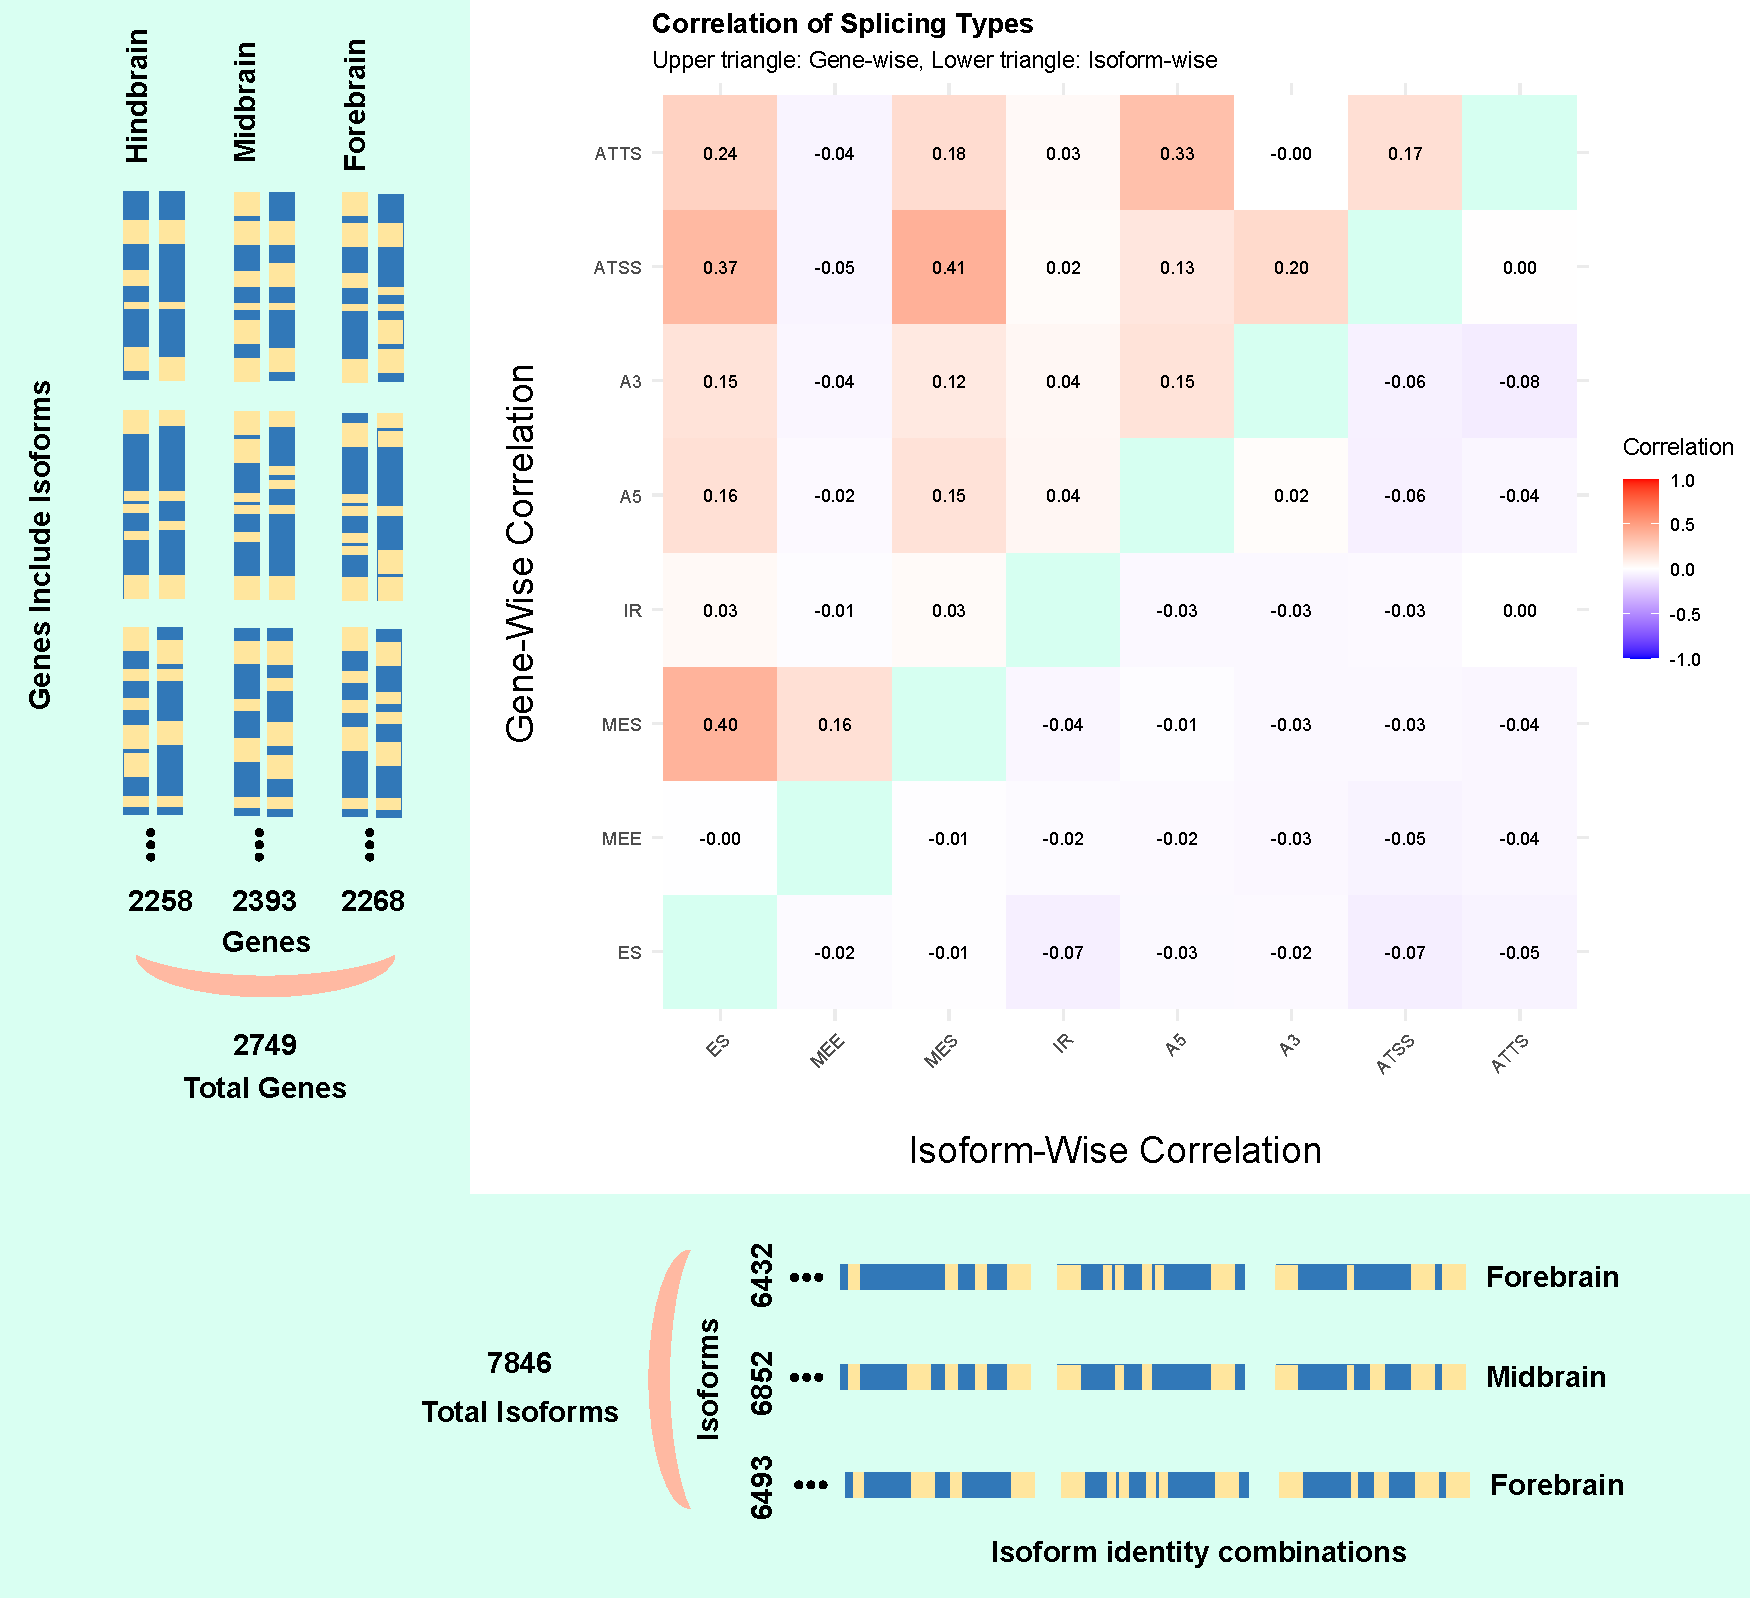
\includegraphics[width=0.84\textwidth]{figure_thesis_splicing_identity.pdf}
\caption{\textbf{Regional transcript-structure event composition and co-occurrence.} The upper-left summary gives the numbers of genes and transcripts meeting the original contrast-wise DTU criteria (q-value $<0.05$ and $|\dIF|\geq0.10$ in at least one of 28 temporal contrasts) in forebrain, hindbrain and midbrain and in their union. The correlation matrix compares co-annotation of event classes at gene level (upper triangle) and within individual transcripts (lower triangle); positive values indicate co-occurrence and negative values mutual avoidance. The lower summary counts recurrent combinations of event annotations among the 7,846 transcripts in the regional union. ES, exon skipping; MEE, mutually exclusive exon; MES, multiple exon skipping; IR, intron retention; A5, alternative 5$'$ splice site; A3, alternative 3$'$ splice site; ATSS, alternative transcript start; ATTS, alternative transcript end. A transcript may carry more than one annotation. Figure retained from the doctoral analysis \citep{gounder_thesis_2025}.}
\label{fig:thesissplicingidentity}
\end{figure}

\subsection{An E15.5-centred discontinuity dominates the midbrain temporal landscape}

Forebrain and hindbrain DTU counts generally increased with the interval between compared stages. Midbrain followed this pattern early in development, but 941 genes showed DTU between E14.5 and E15.5 and 1,011 between E15.5 and E16.5, compared with 104--182 genes in the corresponding forebrain and hindbrain intervals. The complete 28-contrast landscape and all seven adjacent-stage trajectories expose this two-sided peak directly, consistent with a transient redistribution rather than a monotonic late transition (Figure~\ref{fig:temporal}). It persisted across the tested q-value and effect-size thresholds (Supplementary Figure~S1).

\begin{figure}[htbp]
\centering
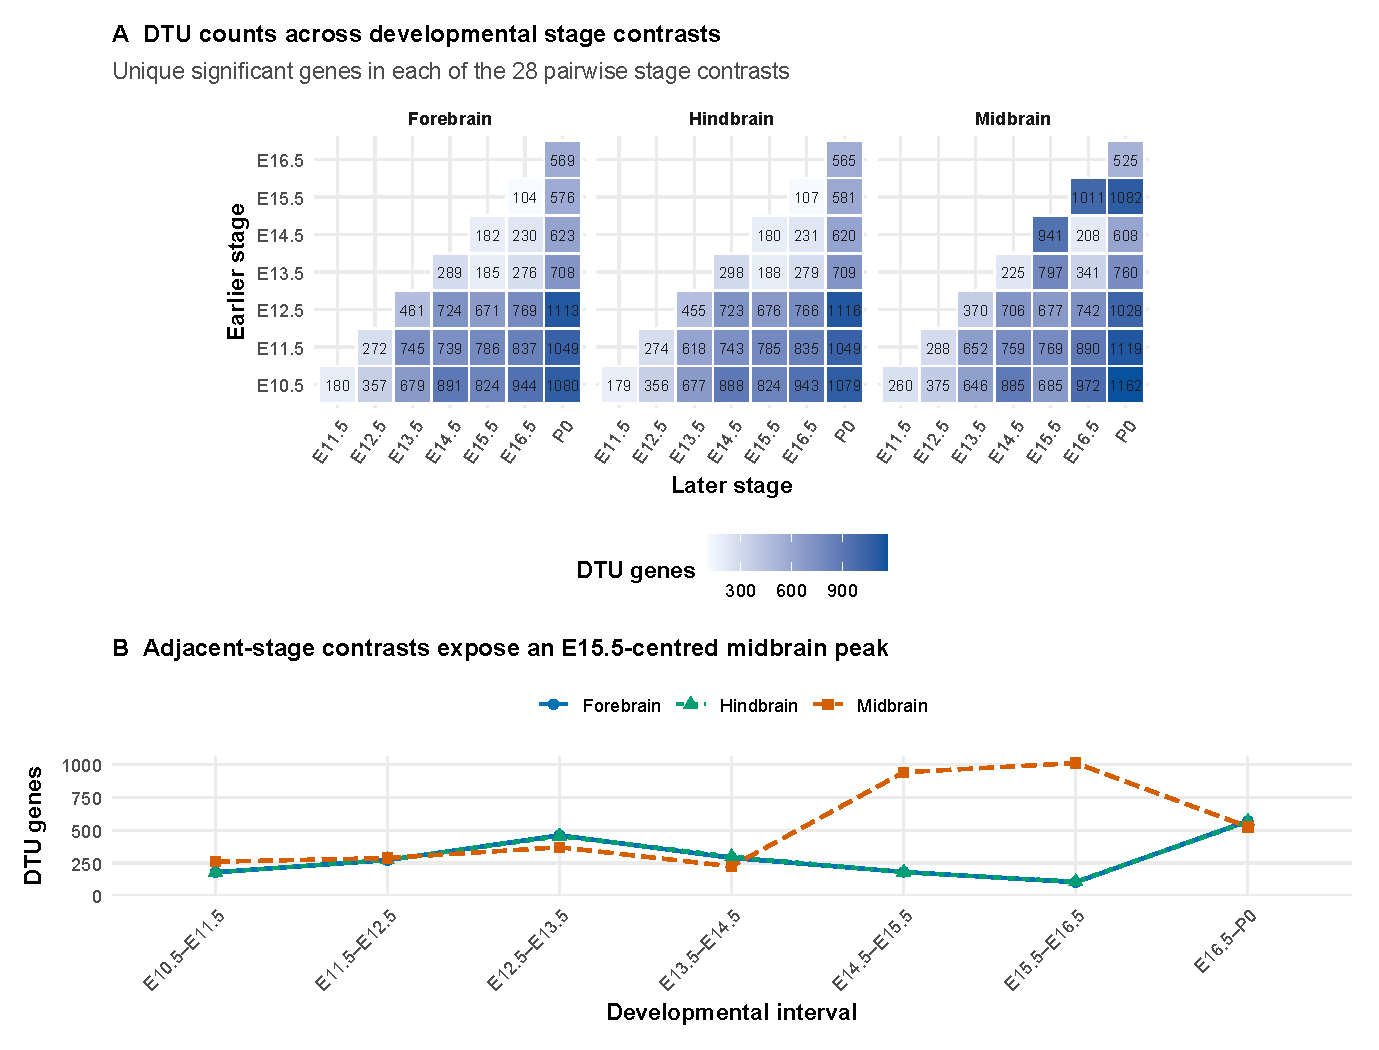
\includegraphics[width=\textwidth]{figure02_repaired_temporal_dtu.pdf}
\caption{\textbf{Complete temporal DTU landscape reveals an E15.5-centred midbrain discontinuity.} (A) Each cell is the number of unique genes meeting the original within-contrast criteria (isoform q-value $<0.05$ and $|\dIF|\geq0.10$) for the indicated earlier and later stage, shown separately for forebrain, hindbrain and midbrain. Cell colour encodes the count and the printed number gives its value. All 28 pairwise contrasts among E10.5, E11.5, E12.5, E13.5, E14.5, E15.5, E16.5 and P0 are included. (B) The same counts for the seven adjacent-stage contrasts; colour denotes brain region. A gene can contribute to more than one contrast. The two midbrain intervals flanking E15.5 contain 941 and 1,011 DTU genes. $\dIF$, between-stage change in relative transcript fraction.}
\label{fig:temporal}
\end{figure}

Both E15.5 midbrain replicates separated from the remaining samples on principal component 2. Public records identify distinct biosamples and libraries, high RNA integrity, and passing depth and concordance metrics, arguing against failure of a single library. However, the two raw files occupied adjacent lanes of one flowcell, and the E14.5--E15.5 interval crosses a documented change from individual-animal to pooled-tissue collection and collection laboratory. The source study itself considered contamination of pooled E15.5/E16.5 material as an explanation for an anomalous profile in another organ \citep{he_mouse_transcriptome_2020}. The E15.5--E16.5 contrast remains high within the pooled workflow, so the boundary alone cannot explain the peak. Because both replicates share collection and sequencing context, replicate separation excludes a single-library failure but not coordinated processing, dissection, composition or quantification effects.

\subsection{Systematic detection resolves 1,348 transient midbrain episodes}

The original analysis represented the temporal feature as 91 visually selected delayed-response isoforms, 20 of which are shown in Figure~\ref{fig:thesisdelayedmain}. These profiles motivated the explicit diverge--reconverge definition used here.

\begin{figure}[htbp]
\centering
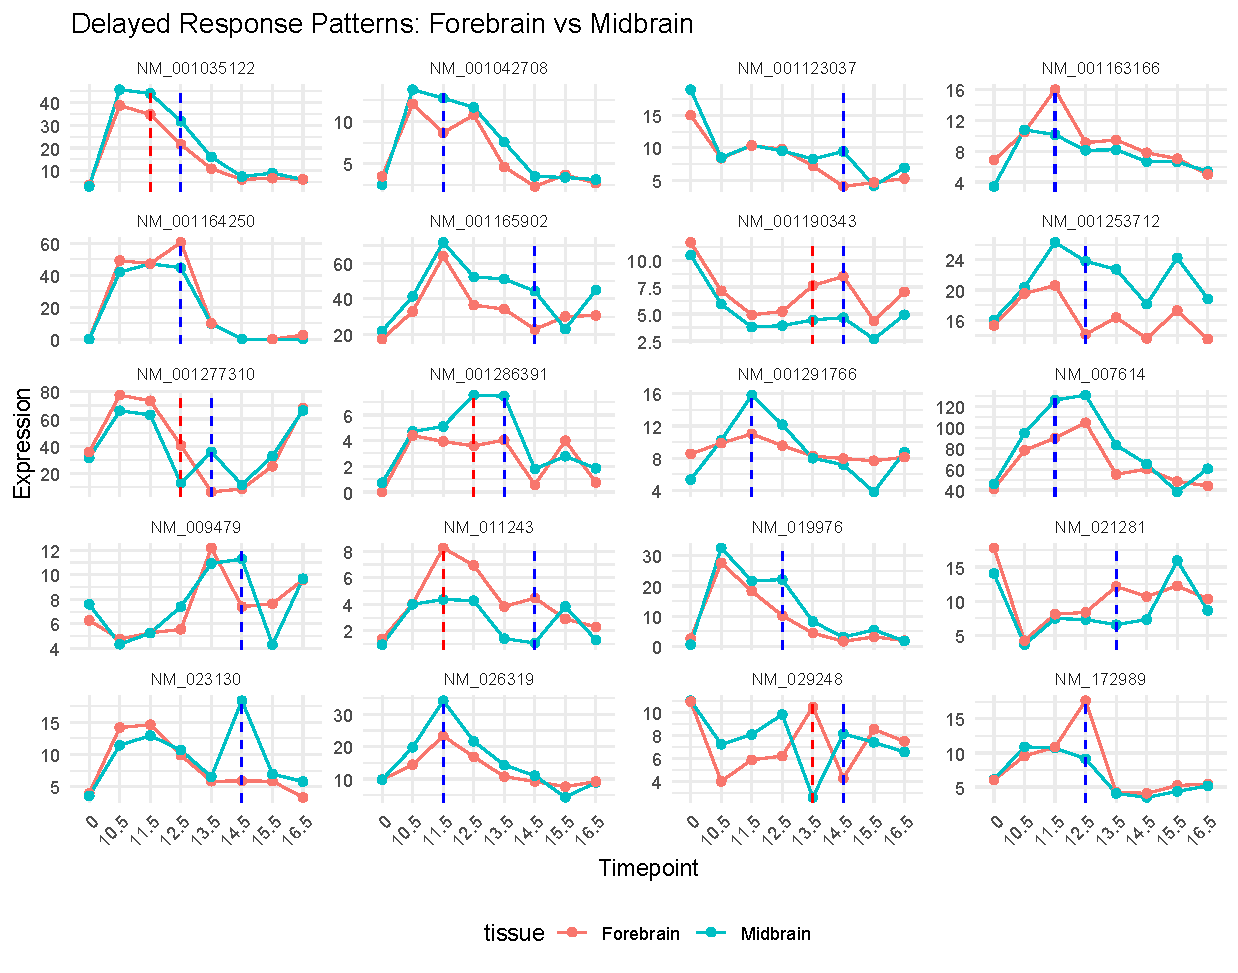
\includegraphics[width=\textwidth]{figureS8_thesis_delayed_response.pdf}
\caption{\textbf{Delayed-response patterns motivating systematic episode detection.} Each facet shows one RefSeq transcript from the original 91-transcript heuristic set. Red and blue lines are the archived forebrain and midbrain expression trajectories, respectively, across E10.5--P0; the vertical dashed lines delimit the interval classified by the original heuristic as divergent. The y-axis is independently scaled archived transcript expression, so amplitudes should be compared across stages within a facet rather than between transcripts. These 20 examples illustrate the temporary separation and subsequent reconvergence that motivated the explicit episode definition; they are descriptive and were not selected by the systematic detector. Figure retained from the doctoral analysis \citep{gounder_thesis_2025}.}
\label{fig:thesisdelayedmain}
\end{figure}

The systematic detector retained 1,348 replicate-consistent candidate episodes in 735 genes. Every episode occurred in midbrain: 1,203 (89.2\%) were confined to E15.5, while 145 began at another stage or spanned a longer interval. Reciprocal higher- and lower-usage isoforms occurred in 1,071 episodes from 490 genes. One-at-a-time threshold changes retained 802--1,588 episodes, and the dependence-robust analysis retained 852 episodes in 474 genes, including the same six programmatically highest-ranked genes (Figures~\ref{fig:framework} and \ref{fig:episodes}). The \texttt{transientDTU} regression reproduced the complete episode table and ordered six-gene panel, establishing that the package implements the paper's decision layer. Supplementary Figure~S3 compares two original heuristic candidates with the systematic output.

The focused satuRn contrast selected 914 transcripts at empirical FDR below 0.05 and 429 genes at DEXSeq-style per-gene q-value below 0.05. Of these genes, 322 belonged to the three-region core and 60 to the threshold-defined midbrain-only set. Thus, a count-model sensitivity analysis using the same abundance estimates detected the specified E15.5 curvature in a substantial subset of genes. Because the contrast was defined for E15.5 after inspection of the data, this analysis did not independently localise the anomaly in time.

\begin{figure}[htbp]
\centering
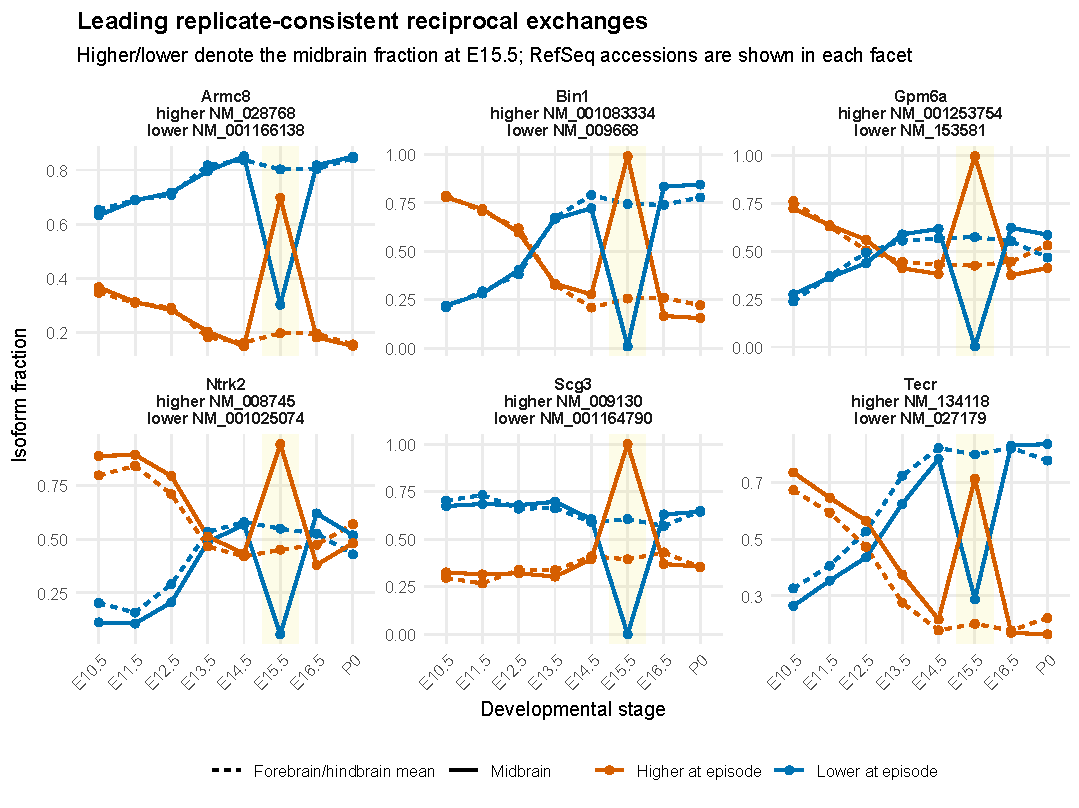
\includegraphics[width=0.90\textwidth]{figureS6_repaired_calibrated_candidates.pdf}
\caption{\textbf{Programmatically highest-ranked reciprocal candidates from the systematic temporal detector.} Each facet shows the stage-mean relative fractions of the two reciprocal transcripts from one selected gene. Solid lines are midbrain means and dashed lines are the mean across forebrain and hindbrain; orange and blue identify the transcript with higher and lower midbrain usage, respectively, at the E15.5 episode. Points are the plotted stage means, and the yellow band marks E15.5. The higher/lower accession pairs are \textit{Ntrk2} NM\_008745/NM\_001025074, \textit{Scg3} NM\_009130/NM\_001164790, \textit{Tecr} NM\_134118/NM\_027179, \textit{Armc8} NM\_028768/NM\_001166138, \textit{Bin1} NM\_001083334/NM\_009668 and \textit{Gpm6a} NM\_001253754/NM\_153581. Facets have independent y-axis ranges. These are the six highest-ranked distinct genes under the deterministic reciprocal-episode ranking described in the Methods; the trajectories are descriptive summaries of the two RNA replicates per region--stage cell.}
\label{fig:episodes}
\end{figure}

Among 1,073 sequence-resolved E15.5 episode isoforms and 4,277 remaining midbrain DTU isoforms, exon skipping occurred in 47.3\% versus 38.2\% (gene-bootstrap prevalence difference 9.1 percentage points, 95\% CI 5.9--12.2), and multiple exon skipping differed by 4.7 points (95\% CI 2.4--7.2). These patterns are compatible with established temporally regulated neural splicing and recent identification of more than 3,000 developmentally regulated AS--NMD exons in mouse and human brain \citep{weyn2018temporal,hu_asnmd_2026}. Alternative starts occurred at similar frequencies (difference 1.2 points, 95\% CI $-1.8$--4.2); alternative ends were modestly enriched (13.0\% versus 10.3\%; difference 2.7 points, 95\% CI 0.4--5.2) but remained a minority.

Median annotated length was 3,616 nucleotides for isoforms higher in midbrain and 3,688 for those lower ($P=0.627$). Across 405 reciprocal genes, the higher-usage product was not systematically shorter (exact sign-test $P=0.318$). Among the sequence-resolved E15.5 episode isoforms, the pattern therefore was not accompanied by a general shift toward shorter higher-usage products.

The six programmatically highest-ranked genes differed across the subsequent evidence axes (Figure~\ref{fig:mechanism}). \textit{Scg3} and \textit{Gpm6a} led the pattern detector, \textit{Bin1} had the largest effect, \textit{Armc8} and \textit{Tecr} had the strongest count-model support, and \textit{Ntrk2} offered the clearest protein-domain interpretation. All 12 expected accession directions persisted across all 512 replicate choices. The panel therefore captures the strongest statistically ranked reciprocal separations while spanning complementary effect-size, model-support and interpretability profiles.

\begin{figure}[htbp]
\centering
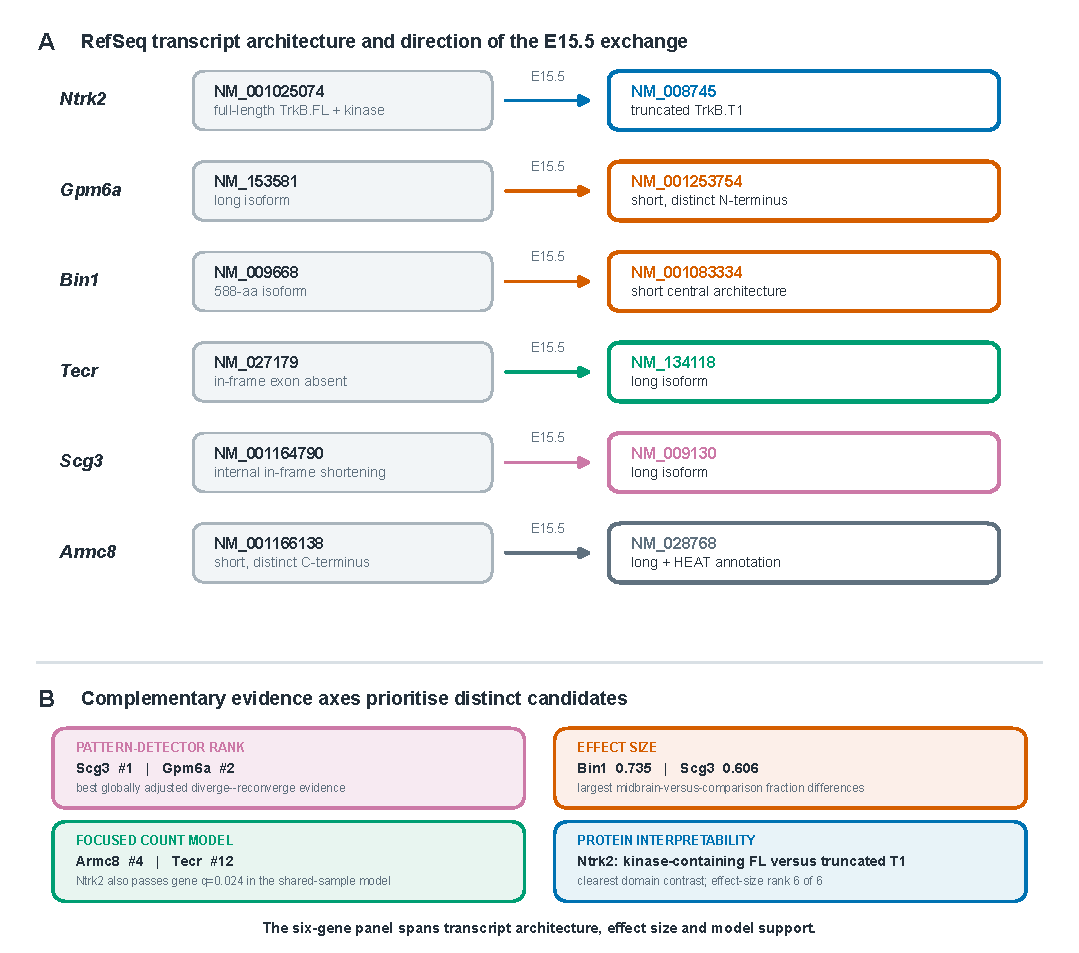
\includegraphics[width=\textwidth]{figure04_repaired_candidate_mechanism.pdf}
\caption{\textbf{Transcript architecture and complementary candidate evidence.} (A) For each of the six reciprocal E15.5 genes, the left box is the RefSeq transcript with lower midbrain fraction and the right box the transcript with higher midbrain fraction; arrows indicate the E15.5 direction of redistribution. Text below each accession summarises the current RefSeq transcript or encoded-protein distinction. (B) Four non-combined evidence axes are reported: rank under the globally adjusted diverge--reconverge detector; maximum absolute midbrain-versus-comparison fraction difference; gene rank among 4,577 genes in the focused satuRn count-model sensitivity analysis; and whether the RefSeq models imply a readily testable protein-domain contrast. Values are not a composite score, and a leading value on one axis does not imply support on the others.}
\label{fig:mechanism}
\end{figure}

Together, the RNA analyses apply the general framework to define an E15.5-centred temporal pattern, resolve it into explicit transcript-level candidate episodes and provide a six-gene experimental panel. As a separate secondary analysis, we then asked whether the full developmental methylation archive provided robust support for proposed regulatory associations.

\clearpage
\subsection{A secondary cross-omic audit evaluates methylation-based prioritisation}

The original workflow reported extensive developmental DMR calling and variation in DMR length, CpG density and temporal overlap in forebrain and midbrain (Figure~\ref{fig:thesisdmrmain}). These descriptive region-level patterns provided context for transcript-level association testing but were not treated as independent evidence for a regulatory mechanism.

\begin{figure}[htbp]
\centering
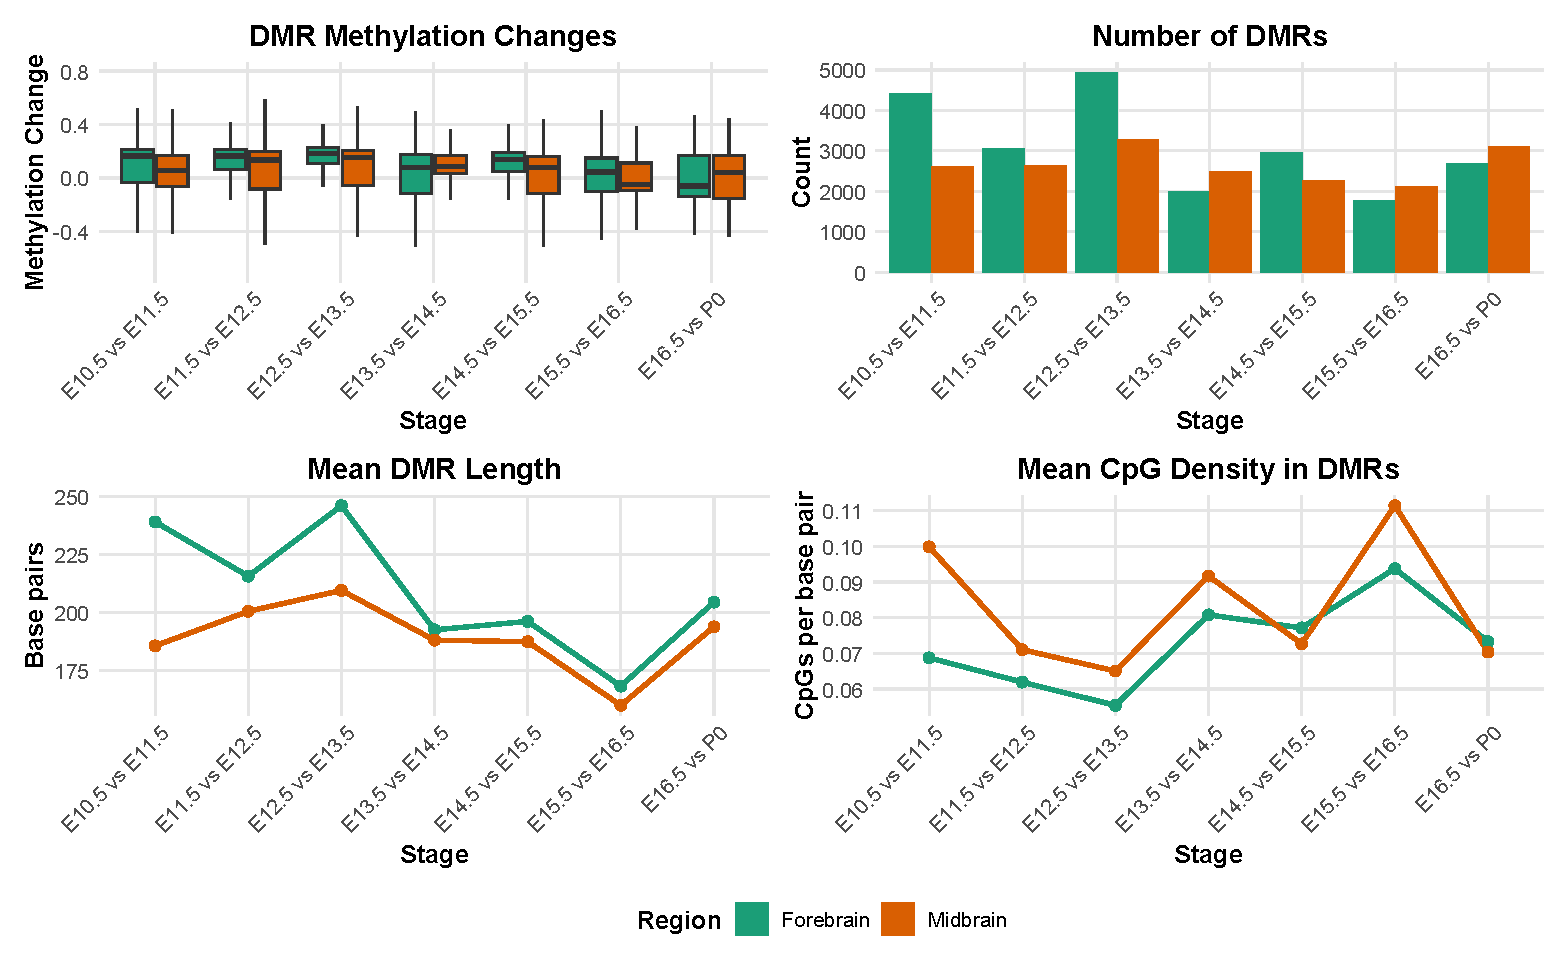
\includegraphics[width=0.88\textwidth]{figureS9_thesis_dmr_overview.pdf}
\vspace{0.4em}
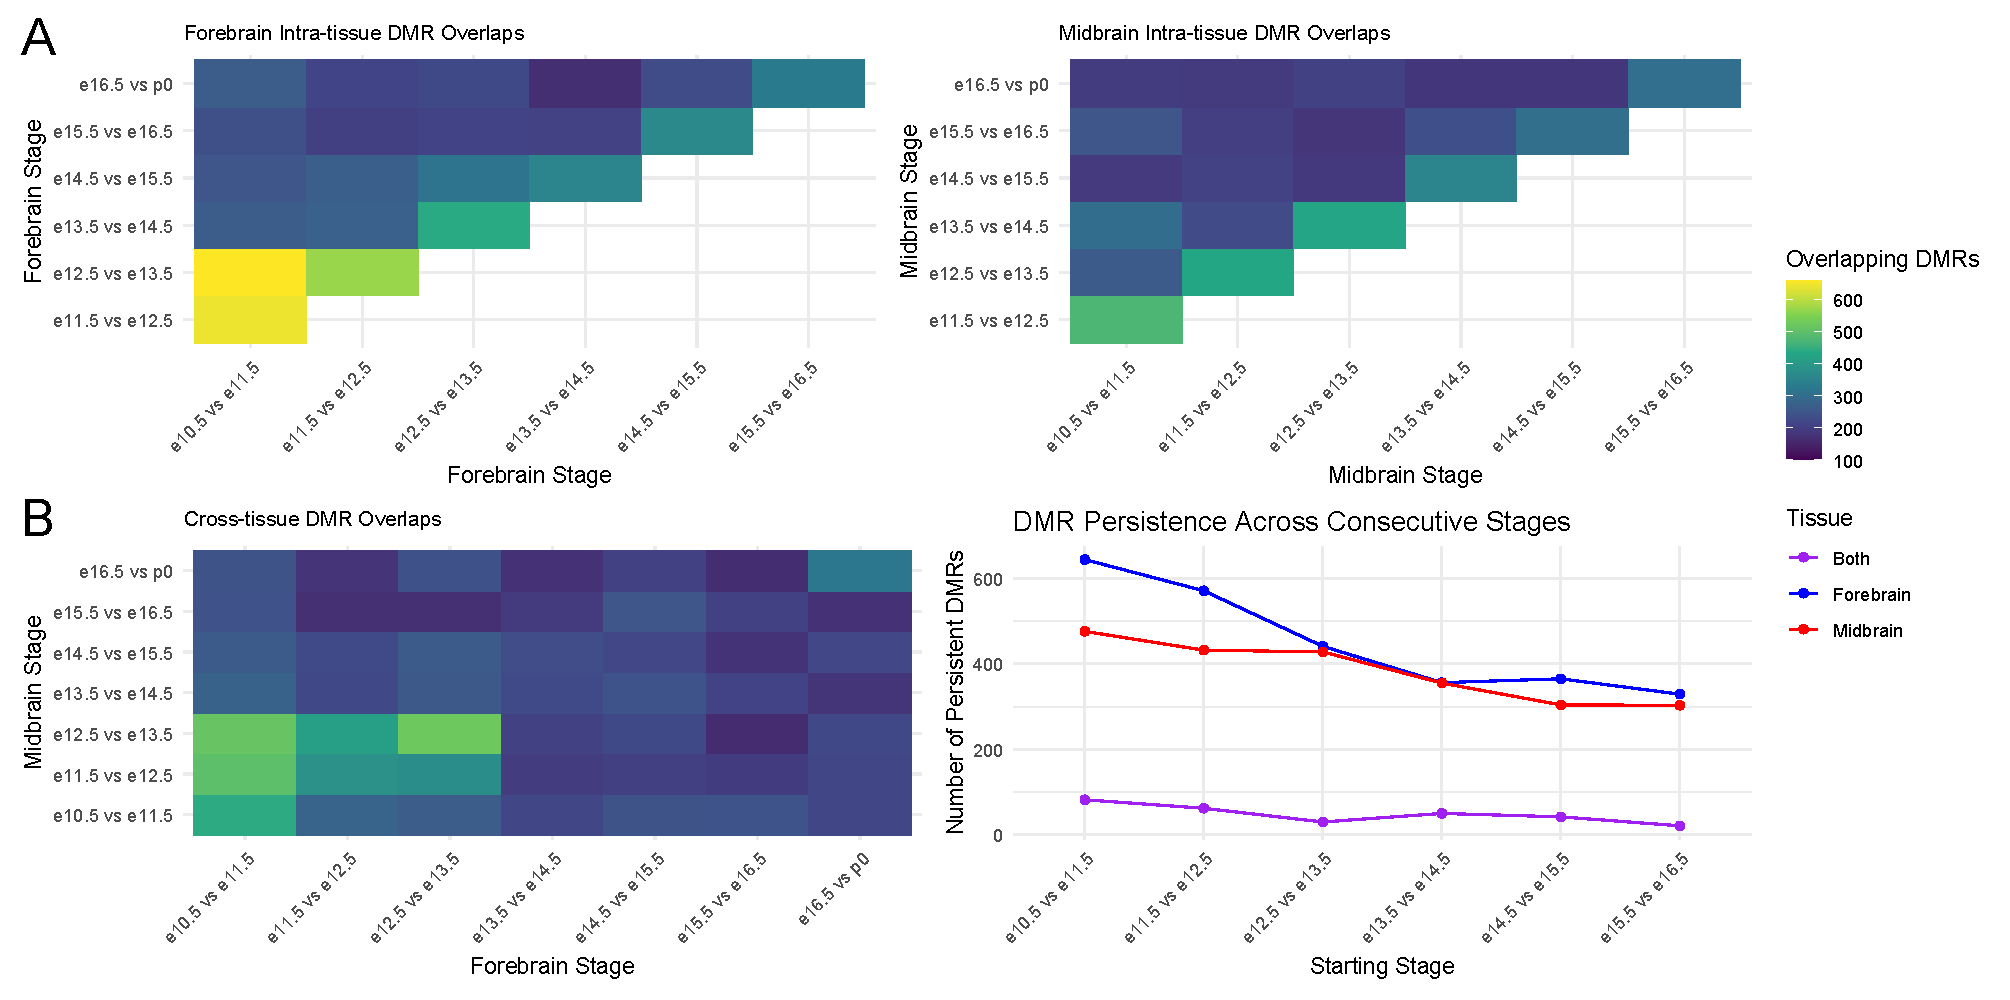
\includegraphics[width=0.92\textwidth]{figureS10_thesis_dmr_temporal.pdf}
\caption{\textbf{Developmental DMR abundance, structure and temporal overlap.} The upper four panels summarise adjacent-stage DMR calls from E10.5--P0 separately for forebrain and midbrain: distributions of methylation change, number of DMRs, mean DMR length in base pairs and mean CpG density in CpGs per base pair. In the lower set, the forebrain and midbrain heatmaps give counts of DMR intervals overlapping between pairs of adjacent-stage call sets, the cross-region heatmap gives overlaps between forebrain and midbrain call sets, and the bar plot counts DMRs persisting across consecutive intervals, classified as forebrain-only, midbrain-only or present in both regions. These are descriptive summaries of the original DMR workflow; colour scales and printed cell values encode overlap counts. Figures retained from the doctoral analysis \citep{gounder_thesis_2025}.}
\label{fig:thesisdmrmain}
\end{figure}

The original workflow used selected-group comparisons, association screens and methylation-weighted rankings to move from epigenomic context to candidate loci (Supplementary Figures~S8--S11). Its archived midbrain correlation table contained 5,635 complete transcript--region tests, each relating stage-mean methylation to relative transcript fraction across eight stages; no row passed the original region-wise false-discovery-rate threshold.

\textit{Shtn1} was the original workflow's most developed example (Figure~\ref{fig:thesisshtn1main}): the reciprocal fractions of RefSeq transcripts NM\_001114312 and NM\_175172 tracked a broad forebrain gene-body methylation profile across development. Because the screen conditioned on selected transcripts and used narrower correction sets, these co-trajectories were treated as hypotheses for the analysis-wide test.

\begin{figure}[htbp]
\centering
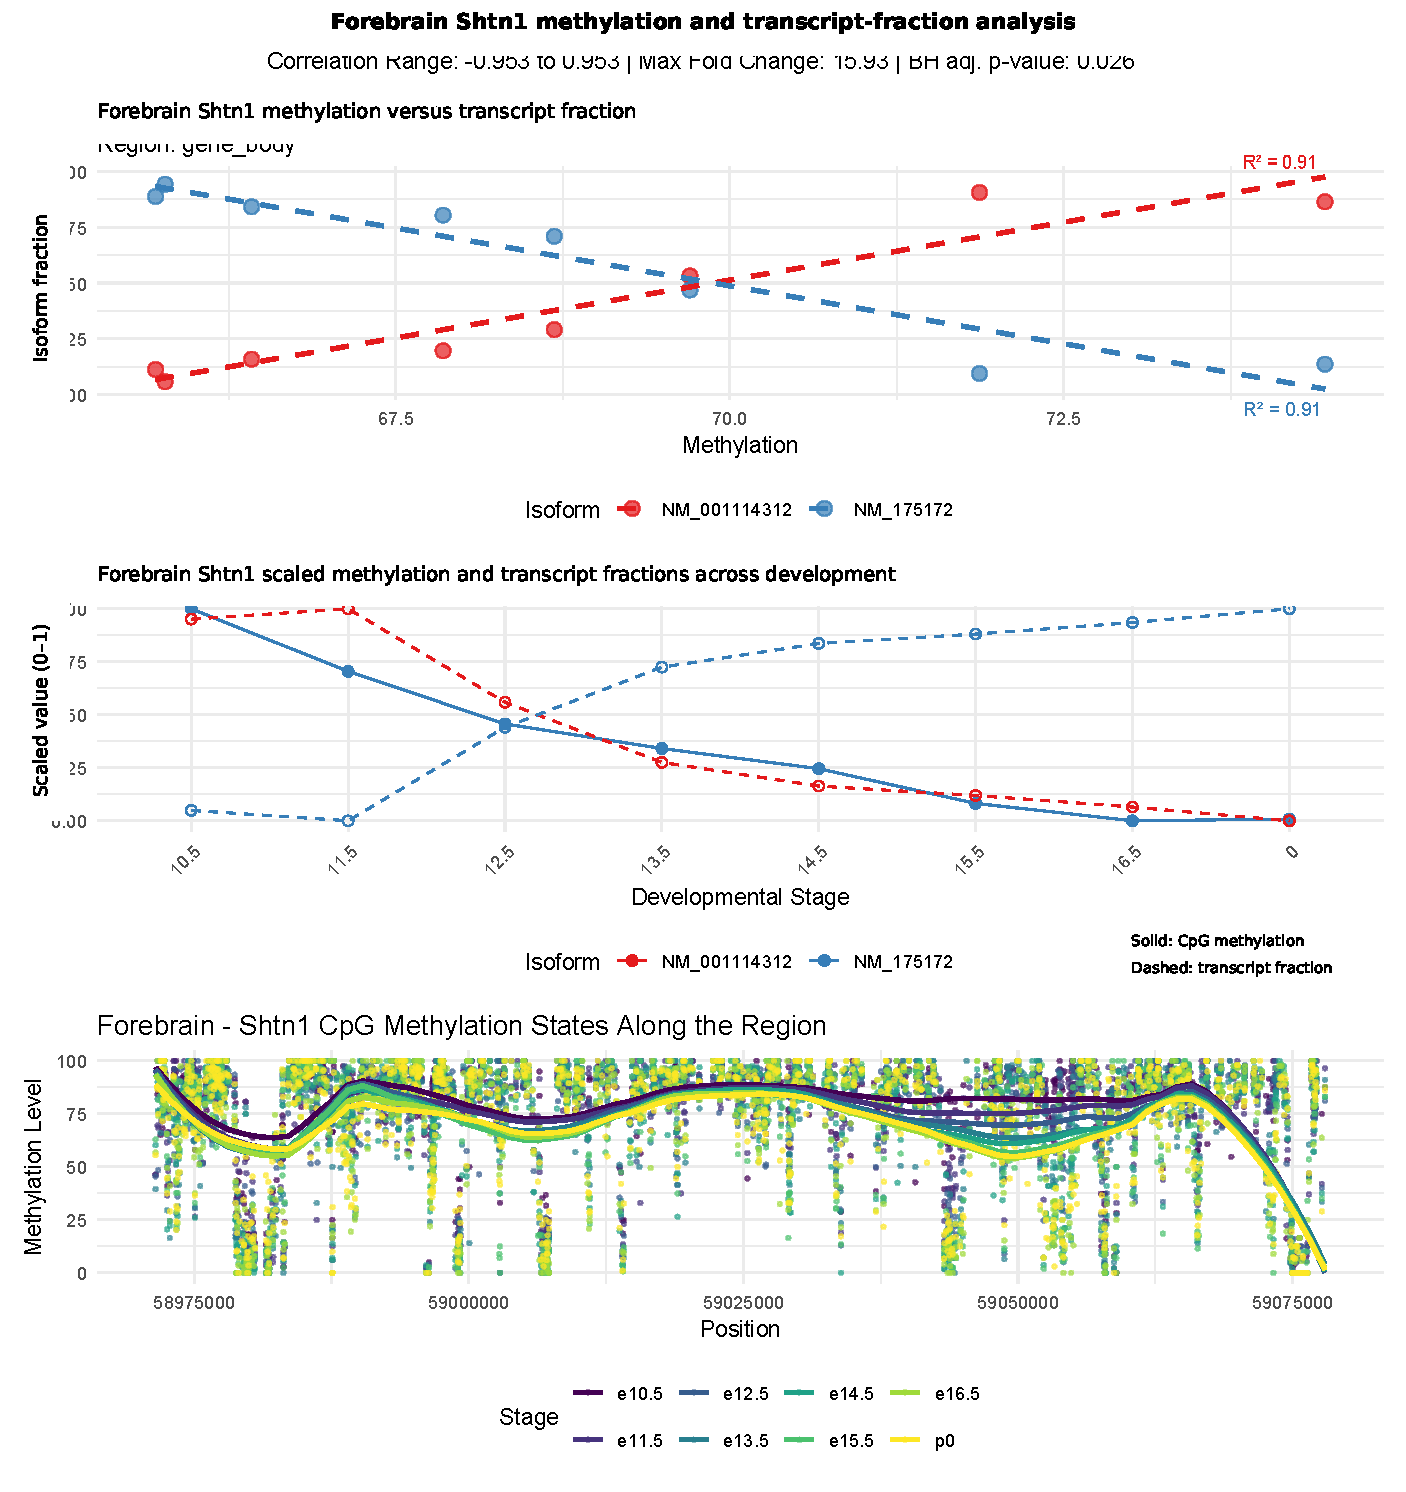
\includegraphics[width=0.92\textwidth]{figureS12_thesis_shtn1.pdf}
\caption{\textbf{Forebrain developmental methylation and transcript usage at \textit{Shtn1}.} The upper panel plots each transcript's stage-mean relative fraction against coverage-weighted methylation across eight developmental stages; NM\_001114312 and NM\_175172 are reciprocal, producing equal $R^2=0.91$ values with opposite correlation directions. The middle panel shows the same stage profiles after each series was scaled to 0--1: solid lines denote methylation and dashed lines transcript fraction. In the lower panel, each point is an individual CpG methylation percentage, coloured by stage, across the approximately 103-kb gene body plus 2-kb margins. The displayed BH-adjusted $P=0.026$ belongs to the original region-wise, prefiltered analysis and is not an analysis-wide result. Data are forebrain; genomic positions use mm10/GRCm38 coordinates.}
\label{fig:thesisshtn1main}
\end{figure}

We therefore evaluated every retained methylation--isoform association under one analysis-wide correction and common sensitivity specifications.

\clearpage
\subsection{Analysis-wide adjustment produces three specification-sensitive parametric screen hits}

The original cross-omic table contained 11,002 tests and 131 region-wise-FDR rows representing 82 genes. Applying one Benjamini--Hochberg correction across all tests to strand-agnostic, coverage-weighted methylation selected three parametric rows at q-value 0.038: the mathematically reciprocal forebrain \textit{Gnao1} transcripts NM\_001113384 and NM\_010308 at the 6-kb upstream window and forebrain \textit{Taok3} transcript NM\_001199685 at the gene body. None overlapped the original 131 rows.

No row passed analysis-wide FDR when methylation was summarised with unweighted CpG means or strand-sensitive overlap. Parametric analyses selected seven detrended rows and one first-difference row, but these sets did not converge on a specification-stable association. Under the exchangeability sensitivity analysis, the smallest stage-label-randomisation q-value was 0.091. Thus, the three primary parametric screen hits depended on the methylation summary and did not meet the specification-stability criterion.

\begin{table}[htbp]
\centering
\small
\caption{\textbf{Analysis-wide calibration of the developmental methylation screen.} Global-FDR rows are counted after adjustment across the complete valid test family for each specification. The archived rows used narrower, prefiltered correction families and are included only as the historical starting point.}
\label{tab:methylation-calibration}
\begin{tabular}{>{\raggedright\arraybackslash}p{0.43\textwidth} >{\centering\arraybackslash}p{0.15\textwidth} >{\raggedright\arraybackslash}p{0.32\textwidth}}
\toprule
Specification & Global-FDR rows & Interpretation \\
\midrule
Archived region-wise, prefiltered workflow & 131 & Historical candidate set; not an analysis-wide family \\
Primary coverage-weighted, strand-agnostic mean & 3 & Two loci: \textit{Gnao1} and \textit{Taok3} \\
Unweighted CpG mean & 0 & Primary rows do not survive \\
Strand-sensitive, coverage-weighted mean & 0 & Primary rows do not survive \\
Linear-detrended parametric profiles & 7 & Different, nonconvergent candidate set \\
Adjacent-stage first differences & 1 & Different, nonconvergent candidate set \\
Stage-label-randomisation sensitivity & 0 & Minimum adjusted q-value 0.091 \\
\bottomrule
\end{tabular}
\end{table}

Among the original 131 rows, 97 retained the same sign in every leave-one-stage-out analysis, 68 had replicate-resampling intervals excluding zero and 57 had unadjusted stage-label-randomisation p-value below 0.05. These stability summaries did not restore overlap with the three analysis-wide parametric screen hits.

\subsection{\textit{Gnao1} shows a bulk developmental transcript redistribution}

Coverage-weighted methylation in the forebrain 6-kb upstream \textit{Gnao1} window fell from approximately 6\% at E10.5 to 1\% at P0. Over the same interval, the relative use of NM\_001113384 fell from approximately 0.24 to 0.01, while NM\_010308 rose reciprocally. The resulting correlations ($r=0.986$ and $-0.986$) are equal and opposite because the two fractions are compositional; they constitute one degree of information, not two confirmations (Figure~\ref{fig:gnao1}).

The coverage-weighted methylation--relative-usage correlation remained strong in the post hoc leave-one-stage-out, detrended and first-difference diagnostics. Absolute expression changed the interpretation: methylation was unrelated to NM\_001113384 abundance ($r=0.008$) but inversely associated with NM\_010308 abundance ($r=-0.908$) and total \textit{Gnao1} expression ($r=-0.911$). The declining NM\_001113384 fraction therefore coincided with expansion of NM\_010308 and the total-expression denominator rather than an observed decline in NM\_001113384. RefSeq annotates distinct 3$'$ coding-exon products, and an independent neuronal-differentiation study reported the same NM\_001113384-to-NM\_010308 developmental change \citep{ncbiGnao1,suzuki2011gnao1}. Recent human iPSC evidence of strong predominance of the NM\_001113384-associated product in astrocytes makes neural/glial composition a locus-specific alternative \citep{volovikov_gnao1_2025}. The data support a reproducible bulk redistribution between the two RefSeq transcripts while leaving its cellular and regulatory basis open.

\begin{figure}[htbp]
\centering
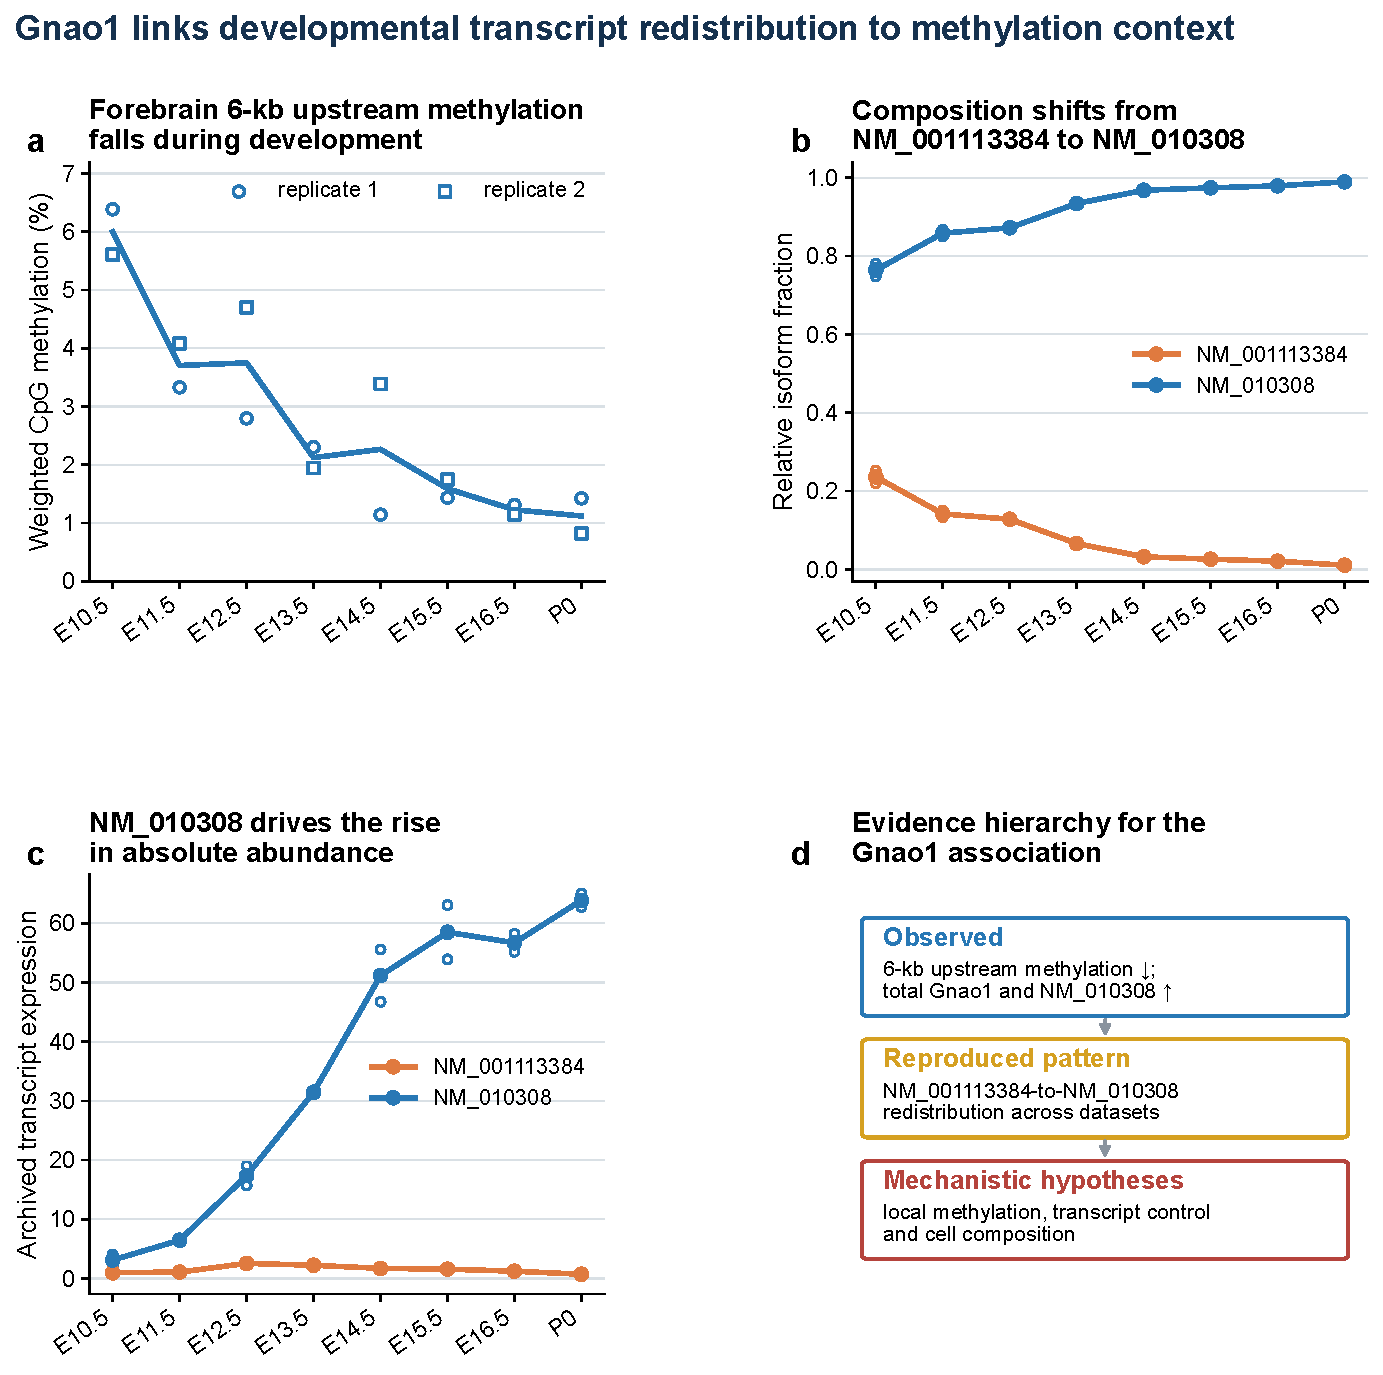
\includegraphics[width=\textwidth]{figure06_repaired_gnao1.pdf}
\caption{\textbf{Forebrain \textit{Gnao1} developmental transcript redistribution and methylation context.} All quantitative panels span E10.5--P0. (A) Coverage-weighted CpG methylation in the archived 6-kb upstream interval on mm10/GRCm38; circles and squares are the two WGBS replicates and the line is their stage mean. (B) Relative fractions of RefSeq NM\_001113384 and NM\_010308; open points are the two RNA replicates and lines are stage means. Because these two retained transcripts exhaust the measured \textit{Gnao1} fraction, their trajectories are mathematically reciprocal. (C) Archived absolute transcript-expression estimates with replicate points and stage-mean lines. NM\_010308 increases with total \textit{Gnao1} expression, whereas NM\_001113384 absolute expression is unrelated to methylation ($r=0.008$, two-sided parametric $P=0.986$ across eight stage means). (D) Summary separating the observed co-trajectories, the independently reported NM\_001113384-to-NM\_010308 developmental redistribution and the untested alternatives of local methylation, transcript regulation and changing cell composition. WGBS and RNA were measured in independent specimens; points are not paired multi-omic observations.}
\label{fig:gnao1}
\end{figure}

The only other parametric locus, \textit{Taok3}, involved RefSeq NM\_001199685 and was temporally coherent but sensitive to methylation summarisation. Its gene-body methylation--usage correlation fell from $r=0.984$ to $r=0.879$ with unweighted CpG means and did not pass analysis-wide FDR; WGBS replicate-profile reliability was 0.343, and methylation was averaged across approximately 159~kb. NM\_001199685 differs from the other validated \textit{Taok3} transcripts in 5$'$ architecture, while the validated variants encode the same protein \citep{ncbiTaok3}, making this a candidate promoter/start-site hypothesis. Overall, the RNA analysis yields an explicit temporal episode set, while the methylation analysis identifies two measurement-sensitive loci for prospective testing without supporting a methylation-mediated mechanism.

\section{Discussion}

The framework addresses a common gap between pairwise DTU testing and the biological question of transient group-specific divergence. Its general contribution is a model-agnostic decision layer that converts statistically supported stage-specific components into explicitly bounded candidate episodes and a reproducible ranking. The accompanying \texttt{transientDTU} package makes this decision layer reusable with explicit input audits, recorded parameters, replicate diagnostics, reciprocal-event annotation and deterministic ranking. In the present application, it resolved the E15.5 midbrain peak into 1,348 transcript-level candidate episodes and the six programmatically highest-ranked reciprocal genes. The concentration of episodes at one developmental stage and their persistence across threshold settings make the pattern a clear target for independent study. A focused count model detected the specified E15.5 curvature in 429 genes, but its post hoc contrast and reuse of the same abundance estimates preclude independent validation.

The structural analysis adds biological resolution to that temporal pattern. Exon skipping was enriched among sequence-resolved E15.5 episodes, whereas alternative starts were not enriched and alternative ends remained a minority. The absence of a general shorter-product bias argues against one simple quantification signature. At the same time, the shared collection and sequencing context of the E15.5 libraries and the expected changes in neural cell composition offer concrete alternative explanations. The functions and cell-type distributions of \textit{Ntrk2}, \textit{Tecr} and \textit{Scg3} make composition especially relevant to the six-gene panel \citep{holt_trkbt1_2019,wang_tecr_2022,gomi_scg3_2021}.

The secondary methylation audit shows why candidate generation and mechanism testing should be separated. Applying one correction across all 11,002 tests produced three parametric rows at \textit{Gnao1} and \textit{Taok3}, but support changed with CpG summarisation (Table~\ref{tab:methylation-calibration}). At \textit{Gnao1}, absolute expression identified expansion of NM\_010308 and total expression rather than loss of NM\_001113384; at \textit{Taok3}, the associated interval was broad and NM\_001199685 shared its encoded protein with the other validated transcripts. These results focus follow-up on transcript composition, promoter or terminal-exon usage and local methylation rather than supporting a general methylation-driven splicing model \citep{batsche2021cd44,chhatbar_mecp2_2020}.

A stronger follow-up should be prospective and modular. The DTU panel requires balanced forebrain, midbrain and hindbrain sampling at E14.5, E15.5 and E16.5 from independent litters, with randomised processing, accession-discriminating assays and long-read confirmation. Cell-resolved or sorted neural, glial and vascular measurements should distinguish within-cell switching from changing composition. For \textit{Gnao1}, local methylation editing should measure total transcription and the NM\_001113384:NM\_010308 ratio separately. For \textit{Taok3}, NM\_001199685-resolved nascent RNA, promoter accessibility and local CpG blocks should be mapped before perturbation. A change in total expression without a ratio change would support a transcriptional-context model; a reproducible ratio change after conditioning on cell state and total expression would support regulation of transcript choice.

The study is limited by the retained source material and sample design. The raw-input manifest, transcript-annotation release and some quantification details were unavailable; the RNA design has two replicates per region--stage cell, and the cross-omic analysis has eight association units. No independent cohort, raw-read reconstruction or analysis-wide junction-level audit was available to establish the origin of the E15.5 pattern. The episode rules and focused satuRn contrast were defined after inspection of the dataset, so the component-test correction does not provide episode-level FDR control. The framework is general at the level of its design requirements and decision rules, but its empirical performance is demonstrated here in one archive; new applications should prespecify thresholds and evaluate operating characteristics for their sampling design and chosen DTU engine. Stage-label randomisation assumes exchangeability and was therefore interpreted only as a sensitivity analysis. Short-read transcript estimates remain vulnerable to identifiability error, while bulk RNA and methylation profiles cannot resolve cell composition \citep{leung_cortex_isoforms_2021,la_manno_brain_atlas_2021,lio_dtu_benchmark_2025,liu_single_cell_methylome_2021}. Conventional WGBS additionally conflates 5mC and 5hmC \citep{huang_bisulfite_5hmc_2010,lister_brain_methylome_2013}.

\section{Conclusions}

This study provides a general post-inference framework for converting stage-specific DTU results and replicate-level transcript fractions into explicit transient transcript-usage candidates, together with its reusable implementation in the R package \texttt{transientDTU}. Applied to developing mouse brain, it identifies 1,348 candidate episodes in 735 genes centred strongly on E15.5, characterises their transcript structure and reports the six programmatically highest-ranked reciprocal genes for independent testing. A separate analysis-wide evaluation of the methylation data produced screen hits at \textit{Gnao1} and \textit{Taok3}, but neither locus was stable across CpG summaries or supported a methylation-mediated mechanism. The framework therefore connects a precisely defined temporal pattern to reproducible experimental prioritisation while preserving the boundary between candidate generation, association and mechanism.

\section*{Abbreviations}

BH: Benjamini--Hochberg; DMR: differentially methylated region; DTU: differential transcript usage; FDR: false-discovery rate; HMM: hidden Markov model; PCA: principal component analysis; WGBS: whole-genome bisulphite sequencing.

\section*{Declarations}

\subsection*{Ethics approval and consent to participate}

Not applicable. This study reanalysed publicly available mouse developmental data and generated no new animal or human-participant data.

\subsection*{Consent for publication}

Not applicable.

\subsection*{Availability of data and materials}

The source RNA-seq and WGBS experiments are publicly available through ENCODE; accession mappings are provided in Supplementary Tables S1 and S3. The planned public repository for analysis code, derived result tables, figure scripts and software-environment records is \url{https://github.com/kohze/developmental-dtu-patterns}. The reusable framework is provided as \texttt{transientDTU} 0.99.1 at \url{https://github.com/Kohze/transientDTU}; its source, documentation, tests, seeded example data and paper-output regression recipe are distributed under the Artistic License 2.0. The article release will record the exact package version and regression-input checksums. A frozen article release with a persistent identifier must be deposited before submission; it will document the provenance and checksums of retained doctoral-analysis objects and the access route for any source object that cannot be redistributed.

\subsection*{Competing interests}

The authors declare no competing interests.

\subsection*{Funding}

This research received no specific grant from any funding agency in the public, commercial or not-for-profit sectors.

\subsection*{Authors' contributions}

Robin Gounder conceived the study, performed the original and current analyses, generated the figures, interpreted the results and drafted the manuscript. Russell Hamilton supervised the research, contributed to interpretation, and reviewed and edited the manuscript. Both authors approved the final manuscript.

\subsection*{Acknowledgements}

The authors thank the ENCODE Consortium for making the developmental RNA-seq and WGBS datasets publicly available.

\section*{Additional files}

\textbf{Additional file 1: Supplementary figures (PDF).} Figures S1--S14 provide threshold and enrichment sensitivities, temporal candidates, transcript characteristics and epigenetic context analyses.

\textbf{Additional file 2: Supplementary Table S1 (CSV).} RNA-seq accessions and library metadata for the 48 analysed region--stage profiles.

\textbf{Additional file 3: Supplementary Table S2 (CSV).} Forebrain--hindbrain matrix-column similarity and source-mapping assessment.

\textbf{Additional file 4: Supplementary Table S3 (CSV).} ENCODE accessions used for the RNA-seq and WGBS provenance assessment.

\bibliographystyle{unsrtnat}
\bibliography{references_dtu_audit,references_methylation_audit}

\ifdefined\submissiononly
\else
\clearpage
\section*{Supplementary figures}
\setcounter{figure}{0}
\renewcommand{\thefigure}{S\arabic{figure}}
\renewcommand{\theHfigure}{S\arabic{figure}}

\begin{figure}[htbp]
\centering
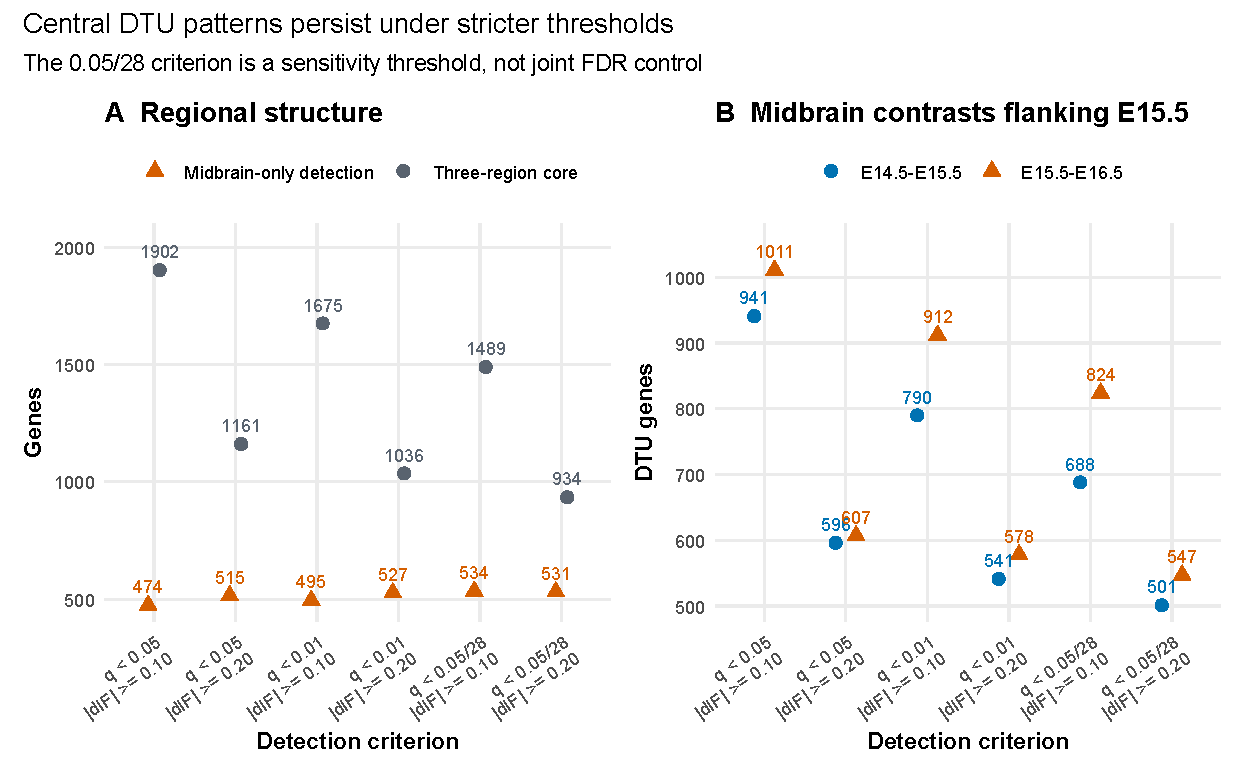
\includegraphics[width=\textwidth]{figureS2_repaired_thresholds.pdf}
\caption{\textbf{Threshold sensitivity of the regional DTU landscape.} Each point is a unique-gene count under the q-value and absolute change in relative transcript fraction ($|\dIF|$) criterion printed on the x-axis; numbers above points give the exact counts. (A) Circles denote genes detected in forebrain, hindbrain and midbrain, and triangles genes detected only in midbrain, after taking the union across all 28 within-region temporal contrasts. (B) Circles and triangles denote genes detected in the E14.5--E15.5 and E15.5--E16.5 midbrain contrasts, respectively. The $0.05/28$ q-value cutoff is a conservative one-at-a-time sensitivity threshold and does not constitute joint FDR control across contrasts.}
\label{fig:thresholds}
\end{figure}

\begin{figure}[htbp]
\centering
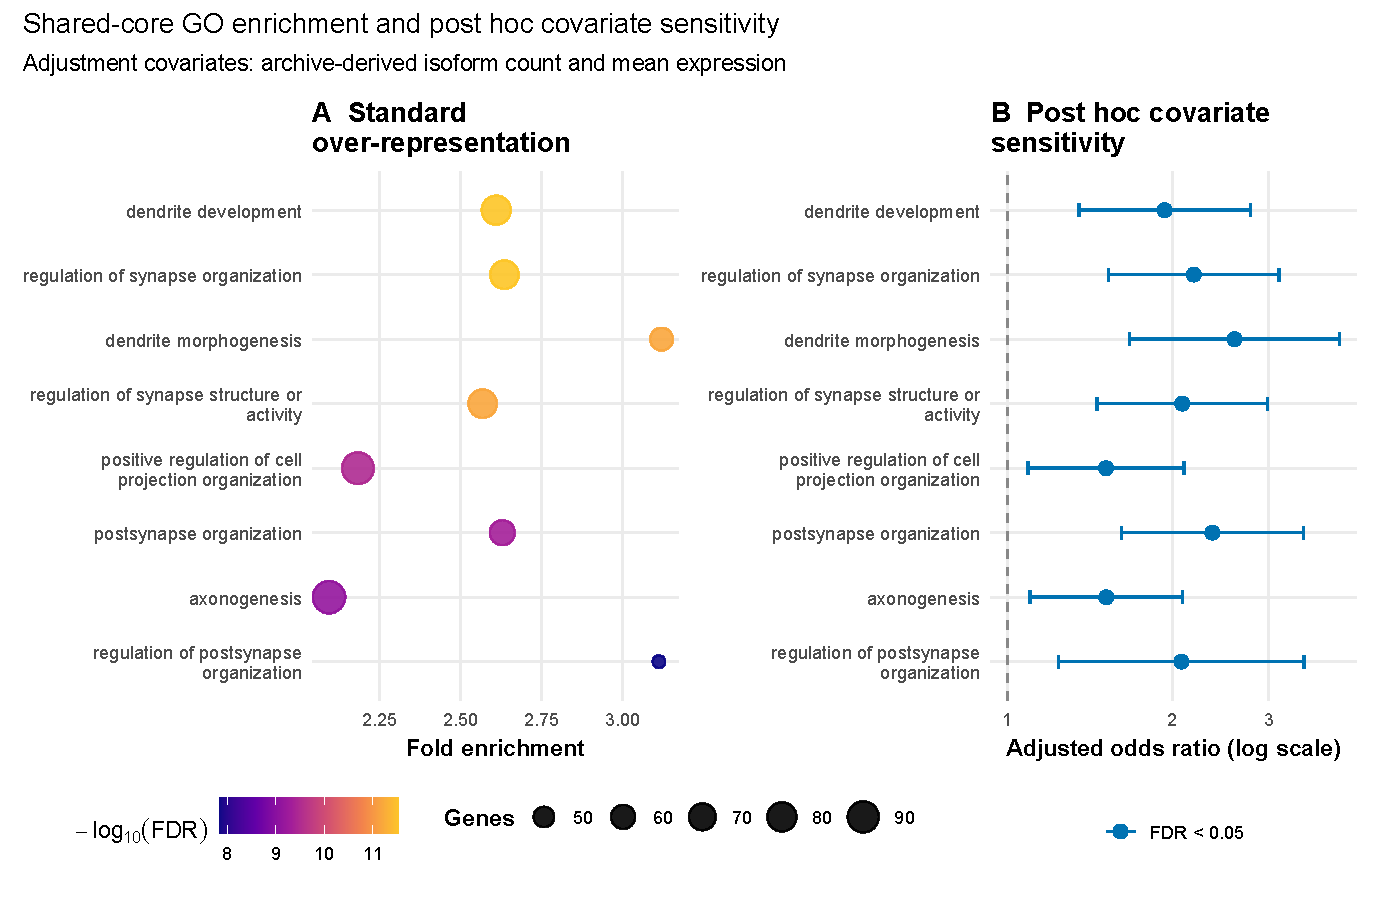
\includegraphics[width=\textwidth]{figureS4_repaired_go_enrichment.pdf}
\caption{\textbf{Shared-core Gene Ontology enrichment and covariate sensitivity.} The analysed set is the 1,902-gene three-region DTU core and the background is the 18,346-gene expressed universe. (A) The eight leading Biological Process terms from the clusterProfiler over-representation analysis. The x-axis is fold enrichment, point size is the number of shared-core genes annotated to the term and colour is $-\log_{10}$ of the Benjamini--Hochberg-adjusted enrichment $P$-value. (B) Post hoc logistic-regression estimates for the same eight terms after adjustment for $\log(1+\text{detectable isoform count})$ and $\log(1+\text{mean expression})$. Points are adjusted odds ratios, horizontal lines are 95\% confidence intervals, the dashed line marks an odds ratio of 1 and blue denotes q-value $<0.05$ after Benjamini--Hochberg adjustment across the eight models.}
\label{fig:go}
\end{figure}

\begin{figure}[htbp]
\centering
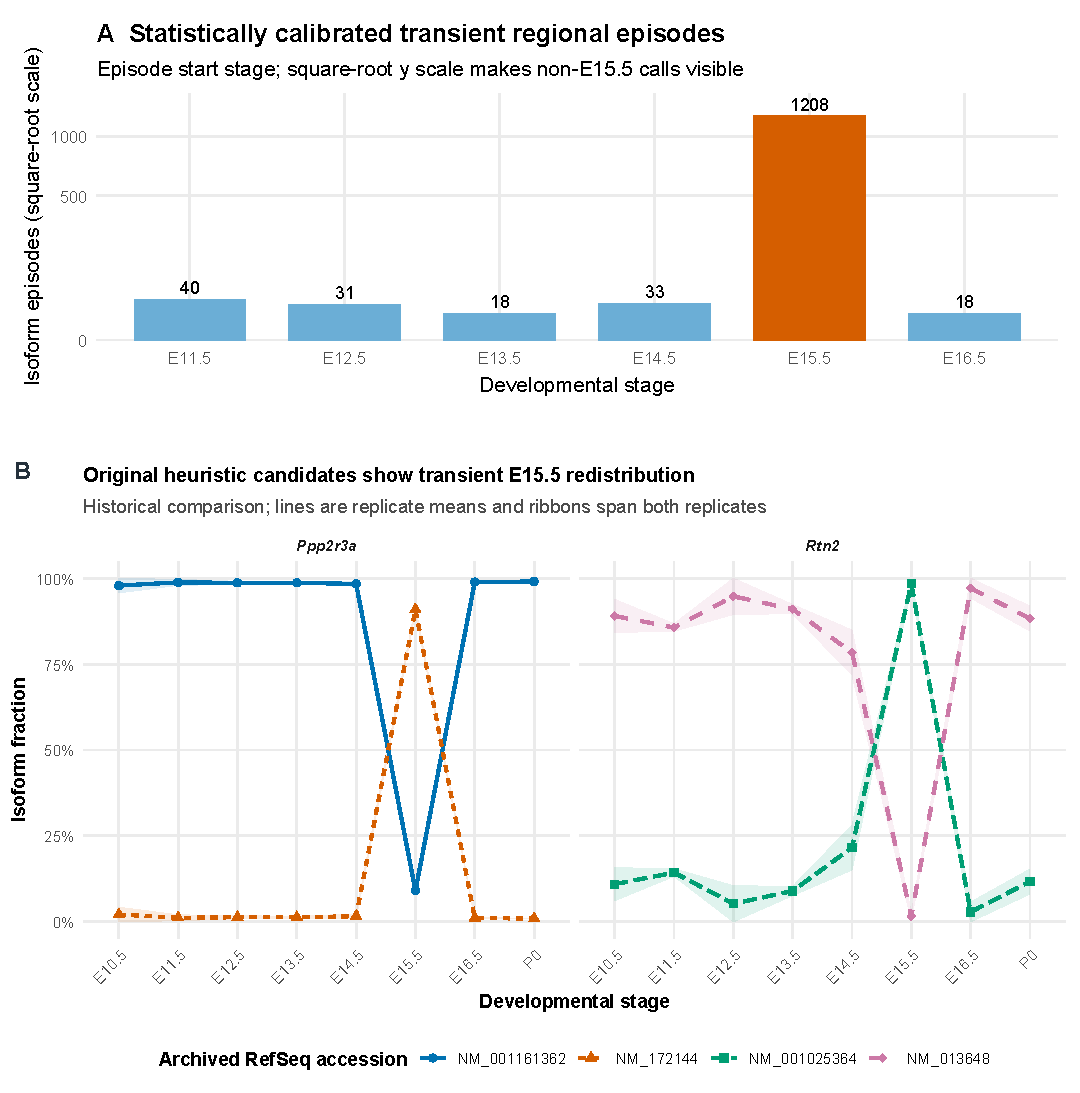
\includegraphics[width=\textwidth]{figure03_repaired_transient_episodes.pdf}
\caption{\textbf{Systematic episodes and original delayed-response examples.} The upper panel gives the number of replicate-consistent diverge--reconverge episodes beginning at each embryonic stage; bar labels are raw counts and the y-axis uses a square-root scale so that non-E15.5 calls remain visible. The middle block shows stage-mean transcript fractions for the six programmatically highest-ranked systematic reciprocal pairs: solid lines are midbrain, dashed lines the forebrain/hindbrain mean, and orange/blue denote the transcript higher/lower in midbrain at E15.5. The higher/lower accessions are \textit{Ntrk2} NM\_008745/NM\_001025074, \textit{Scg3} NM\_009130/NM\_001164790, \textit{Tecr} NM\_134118/NM\_027179, \textit{Armc8} NM\_028768/NM\_001166138, \textit{Bin1} NM\_001083334/NM\_009668 and \textit{Gpm6a} NM\_001253754/NM\_153581. The lower block shows the original heuristic candidates \textit{Ppp2r3a} (NM\_001161362 and NM\_172144) and \textit{Rtn2} (NM\_001025364 and NM\_013648); lines are replicate means and ribbons span the two replicate values. All trajectories cover E10.5--P0 and use relative transcript fraction.}
\label{fig:historicalepisodes}
\end{figure}

\begin{figure}[htbp]
\centering
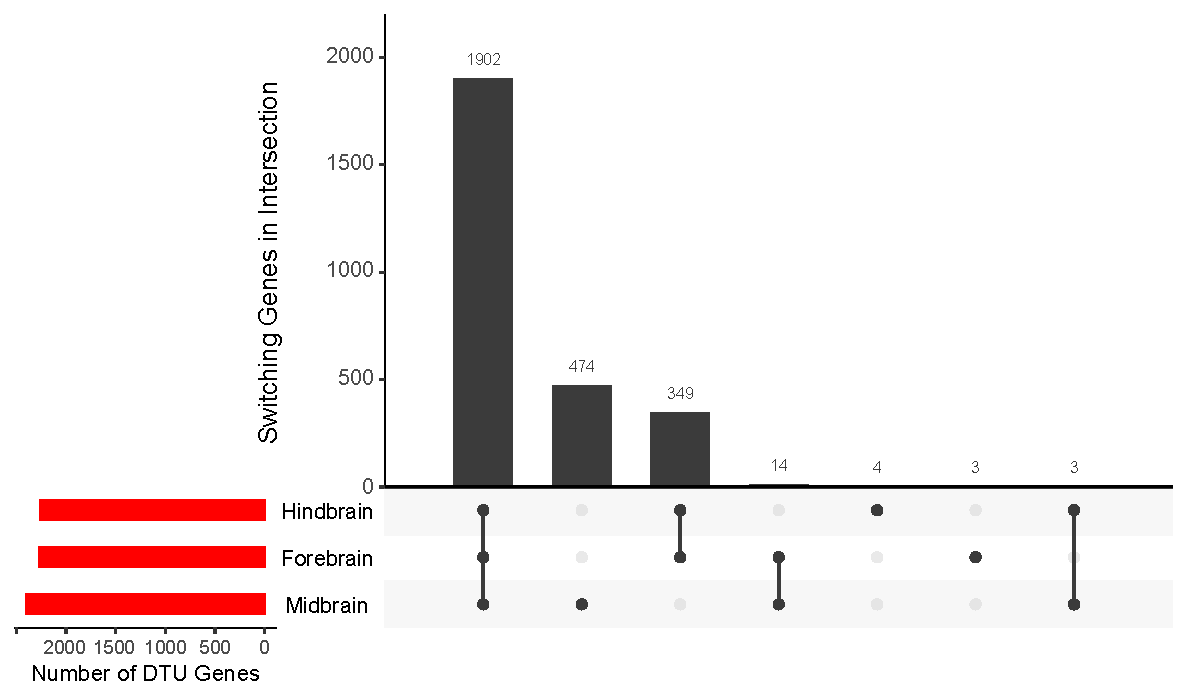
\includegraphics[width=0.88\textwidth]{figure_thesis_dtu_upset.pdf}
\caption{\textbf{Regional intersection of threshold-defined DTU genes.} The sets comprise genes with at least one transcript passing q-value $<0.05$ and $|\dIF|\geq0.10$ in any of the 28 temporal contrasts within forebrain, hindbrain or midbrain. Horizontal bars give total regional set sizes. Filled dots and connecting lines specify each mutually exclusive intersection, and the vertical bar above it gives the number of genes in that intersection. The largest intersection contains 1,902 genes detected in all three regions; 474 genes are detected only in midbrain. A regional set denotes thresholded detection, not strict tissue specificity.}
\label{fig:thesisupset}
\end{figure}

\clearpage
\subsection*{Transcript characteristics and temporal-event summaries}

The following figures present descriptive outputs from the original analysis \citep{gounder_thesis_2025}; inferential results in the main text use the methods specified in this manuscript.

\begin{figure}[htbp]
\centering
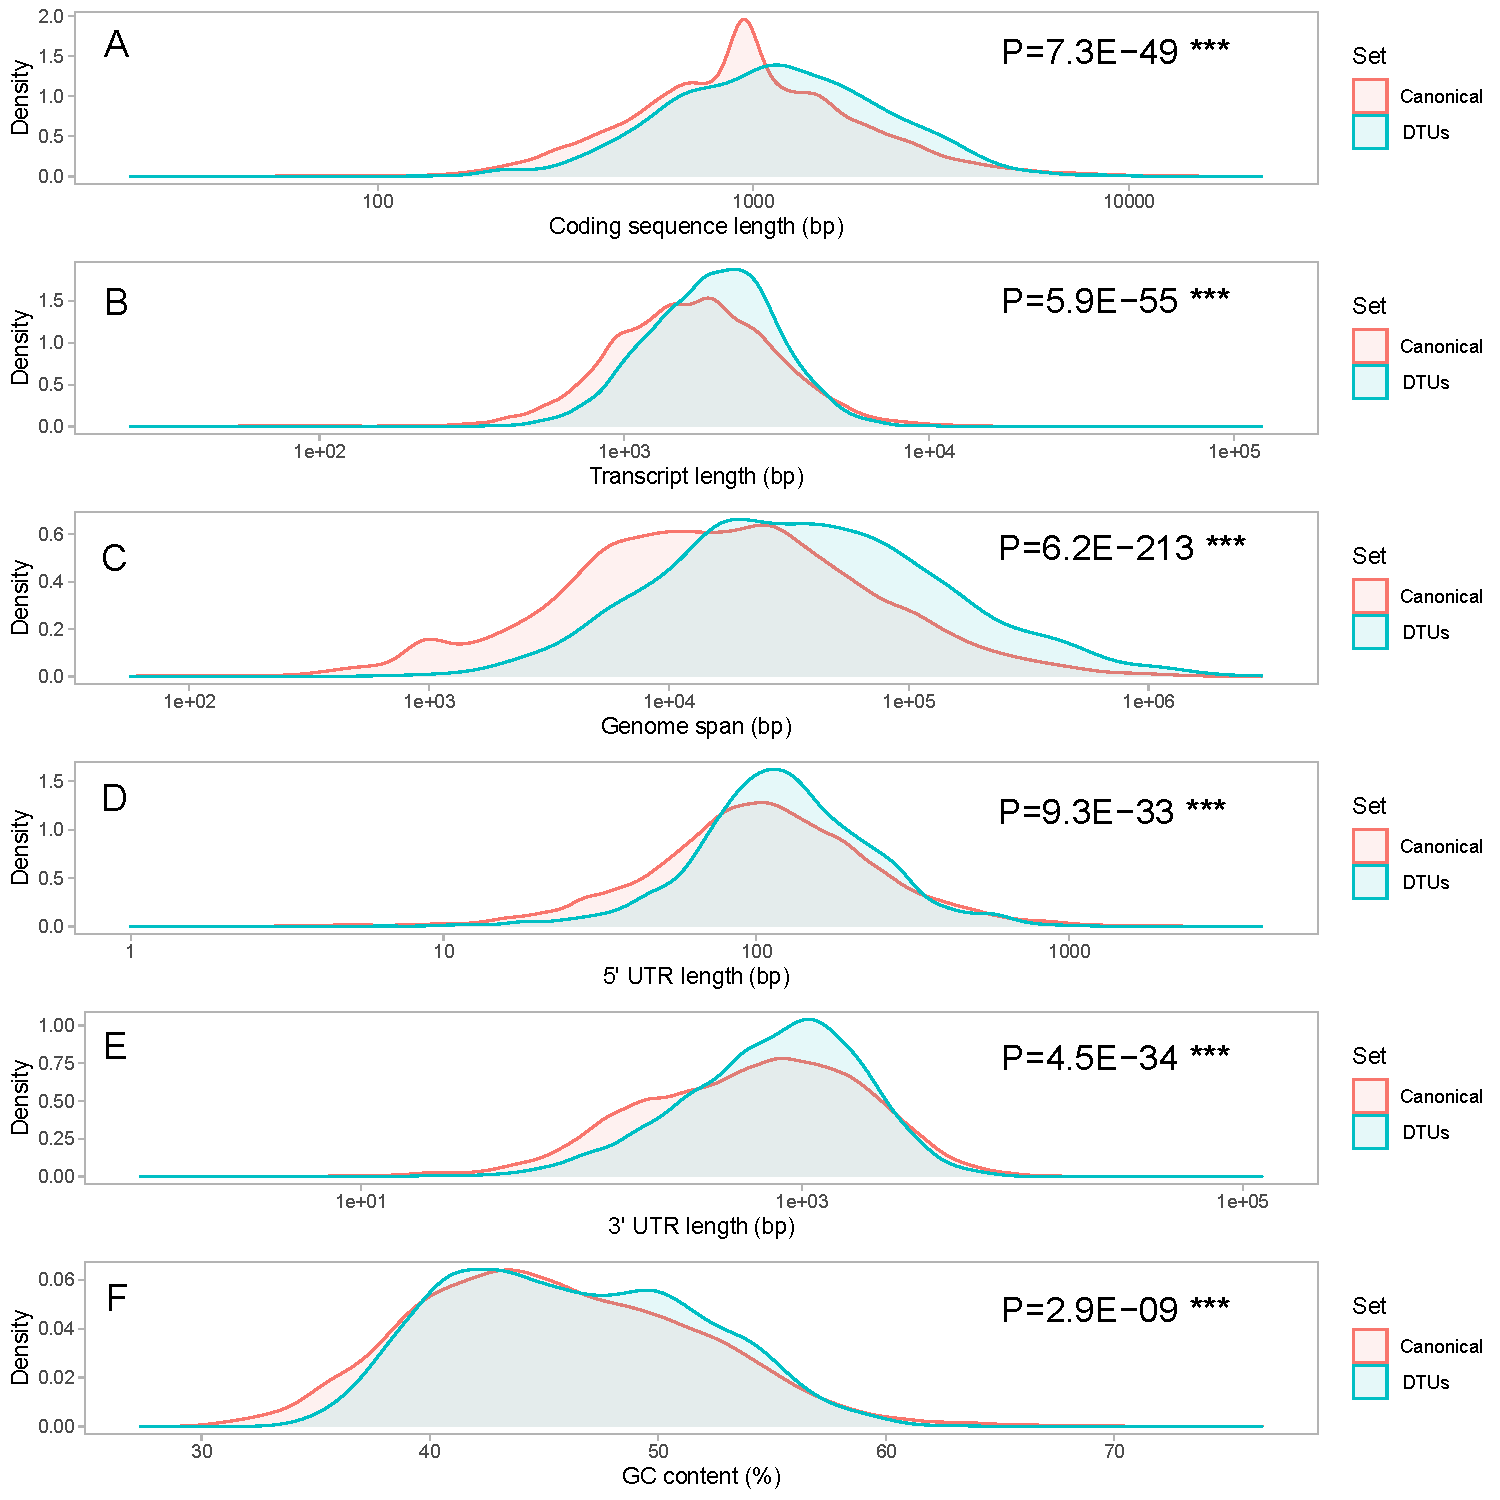
\includegraphics[width=0.80\textwidth]{figureS7_thesis_dtu_attributes.pdf}
\caption{\textbf{Transcript attributes of the DTU catalogue.} Kernel-density distributions compare transcripts in the original threshold-defined DTU catalogue with the original non-DTU comparison universe. Panels show (A) coding-sequence length, (B) total transcript length, (C) genomic span, (D) 5$'$-UTR length, (E) 3$'$-UTR length and (F) GC percentage; length axes are logarithmic where indicated. The $P$-values printed above panels are inherited from the original descriptive workflow; their test identity and multiplicity family were not retained, so they are not used as inferential evidence in the present reanalysis. ``Canonical'' in the inherited legend denotes the non-DTU comparison set rather than a uniquely canonical RefSeq transcript.}
\label{fig:thesisattributes}
\end{figure}

\begin{figure}[htbp]
\centering
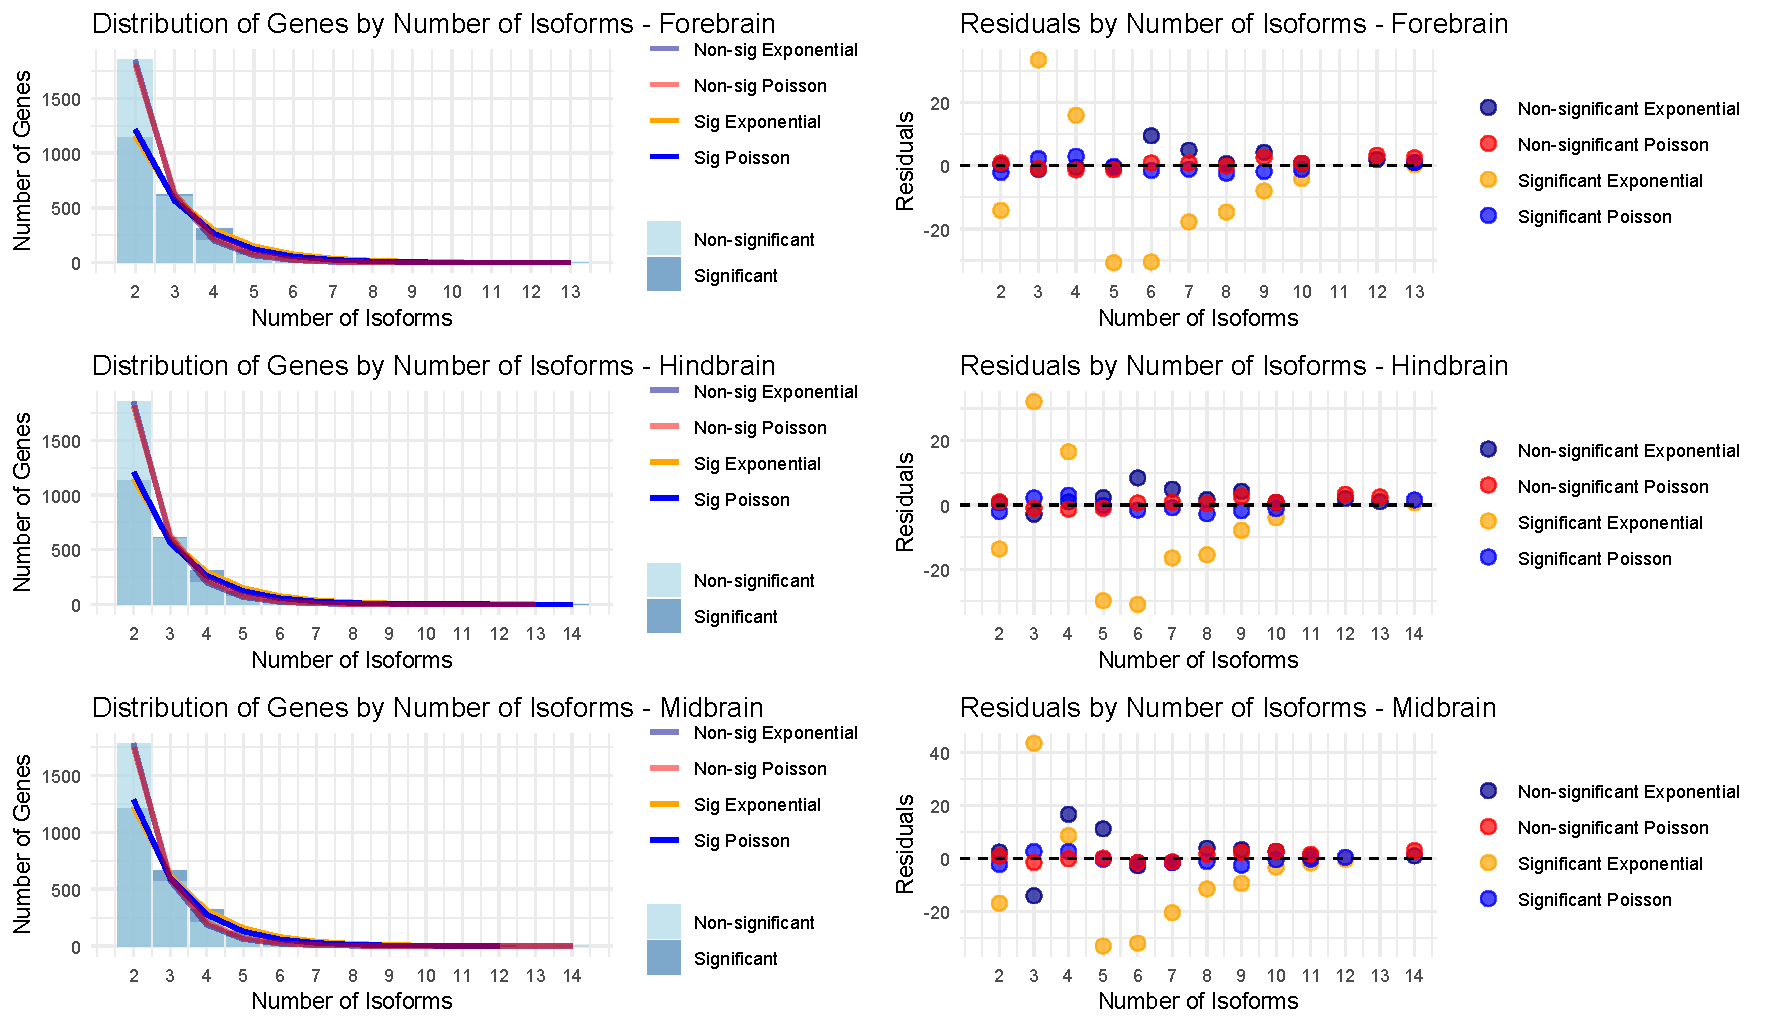
\includegraphics[width=0.84\textwidth]{figure_thesis_isoform_counts.pdf}
\caption{\textbf{Annotated transcript counts in regional DTU and comparison sets.} Rows correspond to forebrain, hindbrain and midbrain. In each row, the left panel gives gene counts by number of annotated transcripts for genes meeting the original regional DTU criteria (``Significant'') and the remaining analysed genes (``Non-significant''); fitted exponential and Poisson curves are overlaid. The right panel shows count residuals from each fitted curve at the same transcript-count values. The display is a descriptive model check of whether genes with more annotated transcripts are over-represented in the DTU catalogue; observations are genes, not individual transcripts.}
\label{fig:thesisisoformcounts}
\end{figure}

\begin{figure}[htbp]
\centering
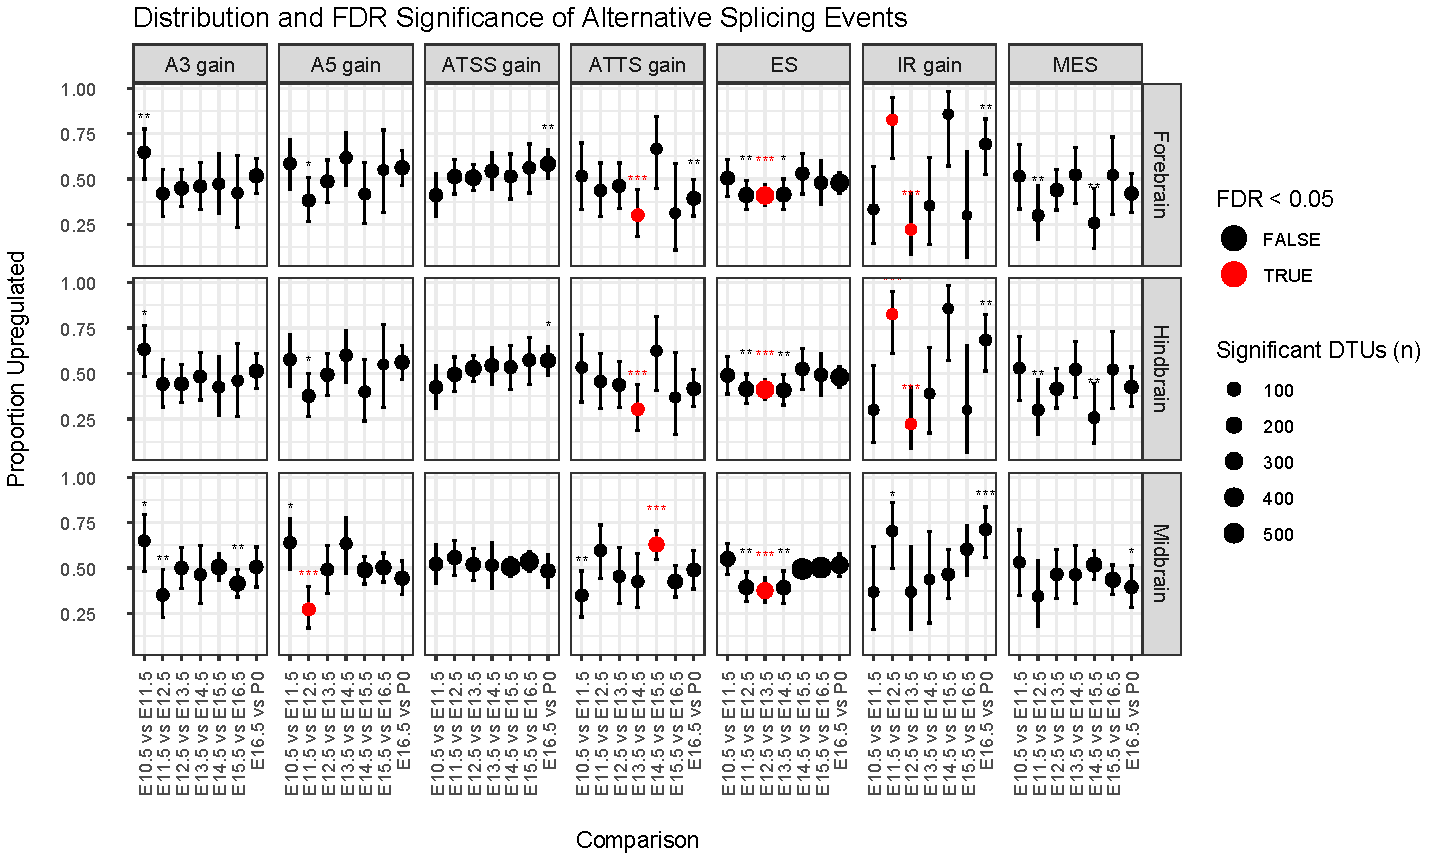
\includegraphics[width=0.86\textwidth]{figure_thesis_temporal_events.pdf}
\caption{\textbf{Temporal distribution of annotated transcript-structure events.} Facets are transcript-structure event classes and the three horizontal groups are forebrain, hindbrain and midbrain. For each adjacent-stage contrast from E10.5--E11.5 through E16.5--P0, a point gives the proportion of significant event-bearing transcripts whose relative usage increased in the stated direction; point size gives the number of significant transcripts and vertical bars are the confidence intervals reported by the original workflow. Red points have the original event-level FDR $<0.05$; asterisks reproduce its significance coding ($*$, $P<0.1$; $**$, $P<0.05$; $***$, $P<0.01$). A3/A5, alternative 3$'$/5$'$ splice-site gain; ATSS/ATTS, alternative transcript start/end gain; ES, exon skipping; IR, intron-retention gain; MES, multiple exon skipping. Event annotations are non-exclusive, and the plot is descriptive rather than part of the systematic episode test.}
\label{fig:thesistemporalevents}
\end{figure}

\begin{figure}[htbp]
\centering
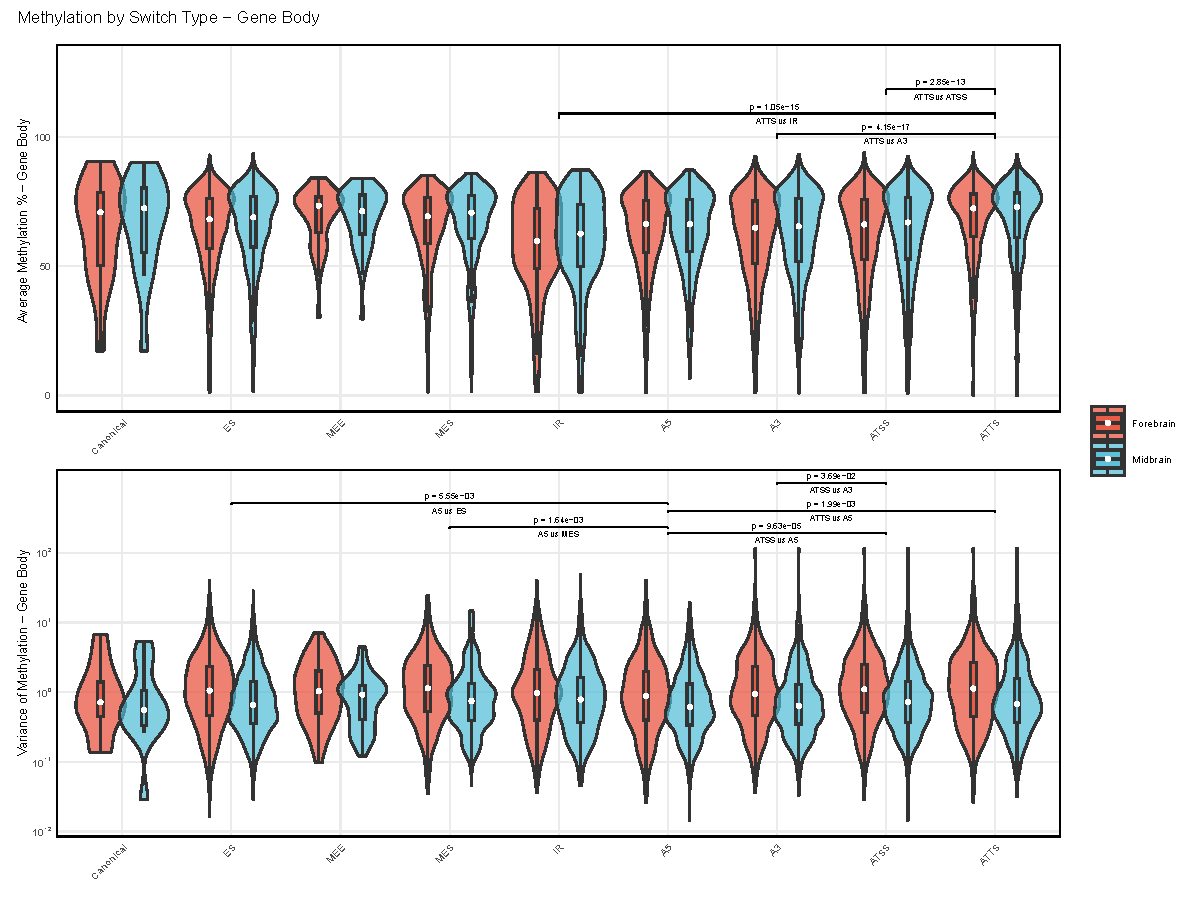
\includegraphics[width=0.90\textwidth]{figureS11_thesis_switch_methylation.pdf}
\caption{\textbf{Gene-body methylation by transcript-event annotation.} Each violin shows the distribution across transcripts in the original selected set, with forebrain and midbrain distinguished by colour. The upper panel uses each transcript's mean gene-body CpG methylation percentage; the lower panel uses its between-sample methylation variance on a logarithmic scale. Groups are ES, MEE, MES, IR, A5, A3, ATSS and ATTS as defined in Figure~\ref{fig:thesissplicingidentity}; annotations are non-exclusive. ``Canonical'' is the inherited label for the comparison group lacking the listed alternative-event annotation, not a uniquely designated RefSeq transcript. Brackets and printed $P$-values are pairwise comparisons from the original workflow and were not included in the analysis-wide methylation correction used in the main text.}
\label{fig:thesisswitchmeth}
\end{figure}

\begin{figure}[htbp]
\centering
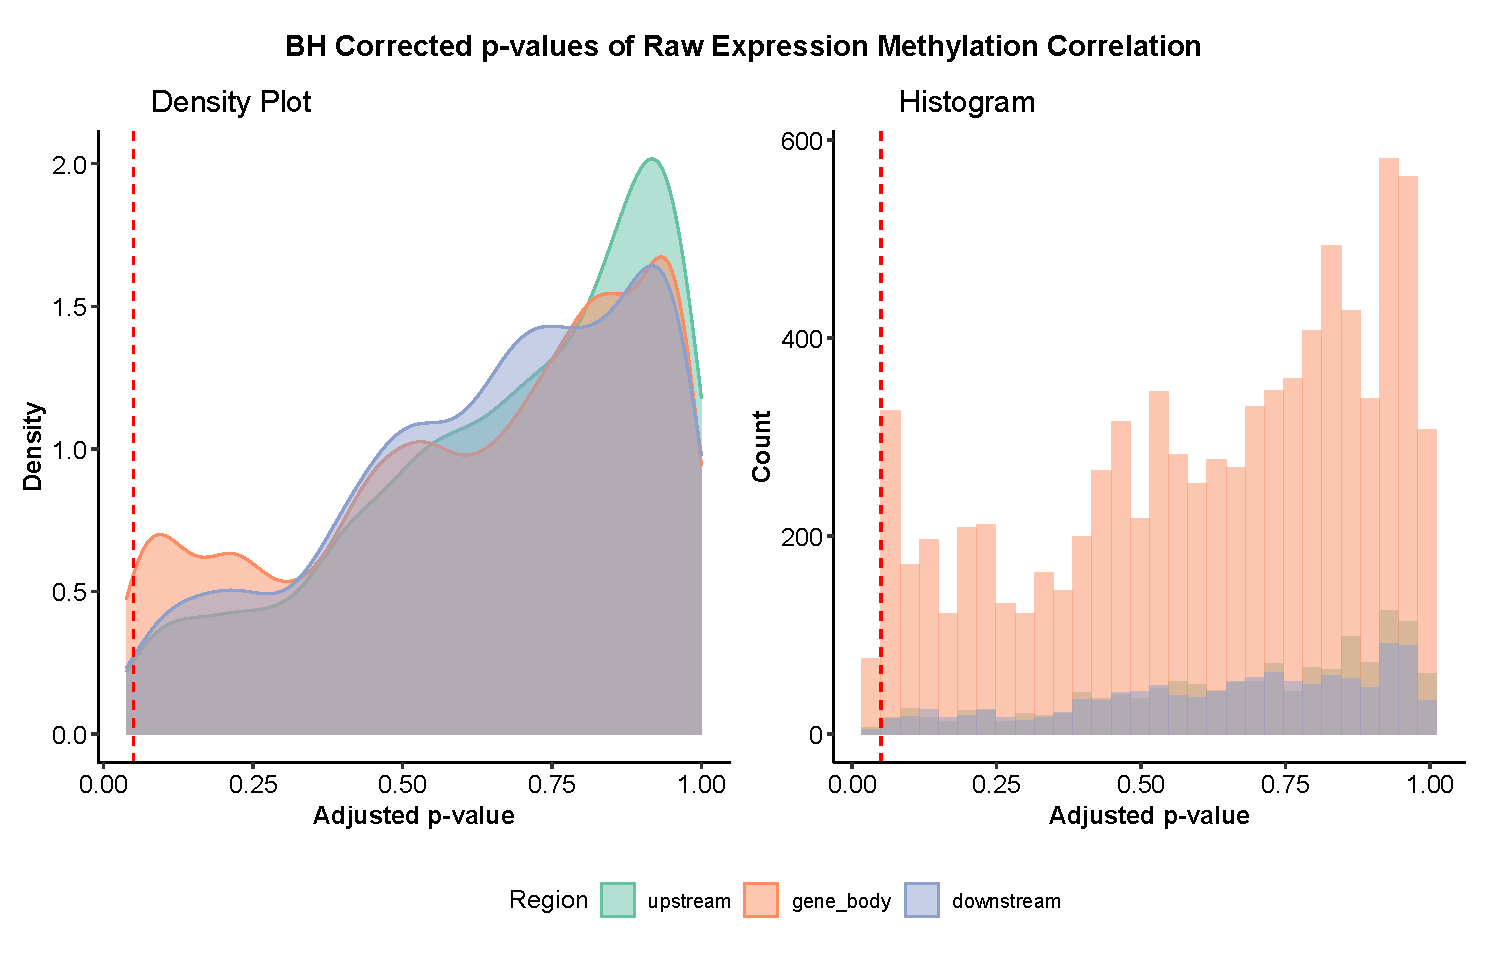
\includegraphics[width=0.90\textwidth]{figure_thesis_archived_bh.pdf}
\caption{\textbf{Methylation associations with absolute transcript expression in the original workflow.} The displayed observations combine forebrain and midbrain transcript--region associations that were prefiltered at nominal correlation $P<0.05$. The left panel is a kernel-density estimate and the right panel the corresponding histogram of Benjamini--Hochberg-adjusted $P$-values; colour denotes the 6-kb upstream window, gene body with 2-kb margins or 6-kb downstream window. Adjustment was performed separately within each genomic-region class after nominal prefiltering. Consequently, these values are conditional, region-wise summaries and are not the analysis-wide q-values reported in the main reanalysis.}
\label{fig:thesisrawbh}
\end{figure}

\begin{figure}[htbp]
\centering
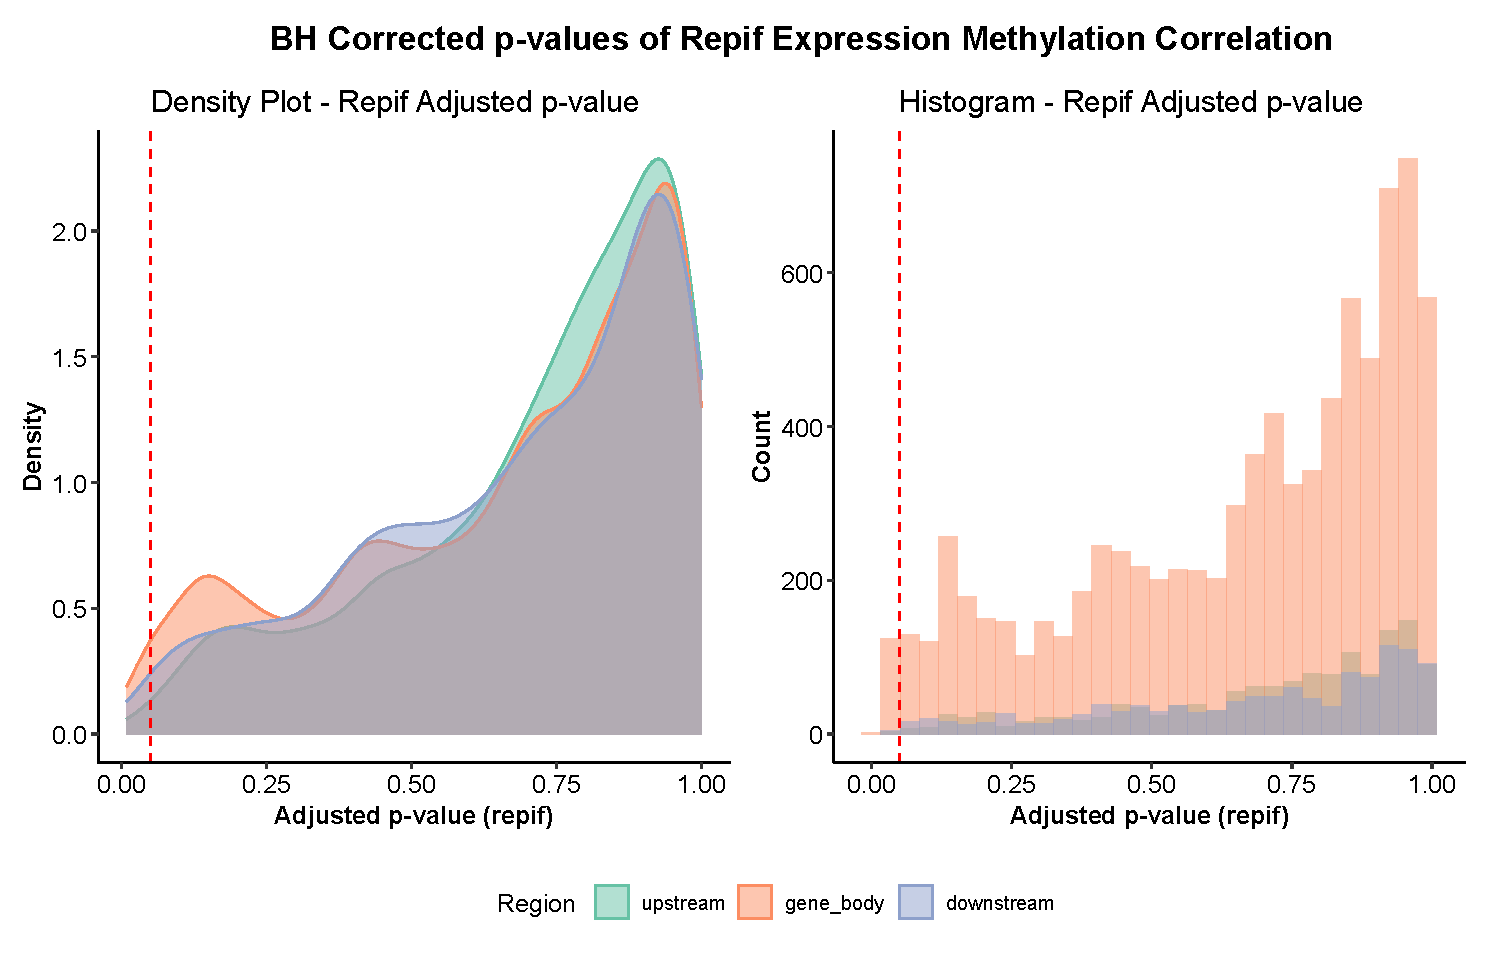
\includegraphics[width=0.90\textwidth]{figure_thesis_archived_repif_bh.pdf}
\caption{\textbf{Methylation associations with relative transcript fraction in the original workflow.} The displayed observations combine forebrain and midbrain transcript--region associations that were prefiltered at nominal correlation $P<0.05$. The left panel is a kernel-density estimate and the right panel the corresponding histogram of Benjamini--Hochberg-adjusted $P$-values; colour denotes the 6-kb upstream window, gene body with 2-kb margins or 6-kb downstream window. Adjustment was performed separately within each genomic-region class after nominal prefiltering. Relative transcript fraction is the transcript abundance divided by the summed abundance of retained transcripts from the same gene. These conditional, region-wise values are distinct from the analysis-wide q-values in the main reanalysis.}
\label{fig:thesisrepifbh}
\end{figure}

\begin{figure}[htbp]
\centering
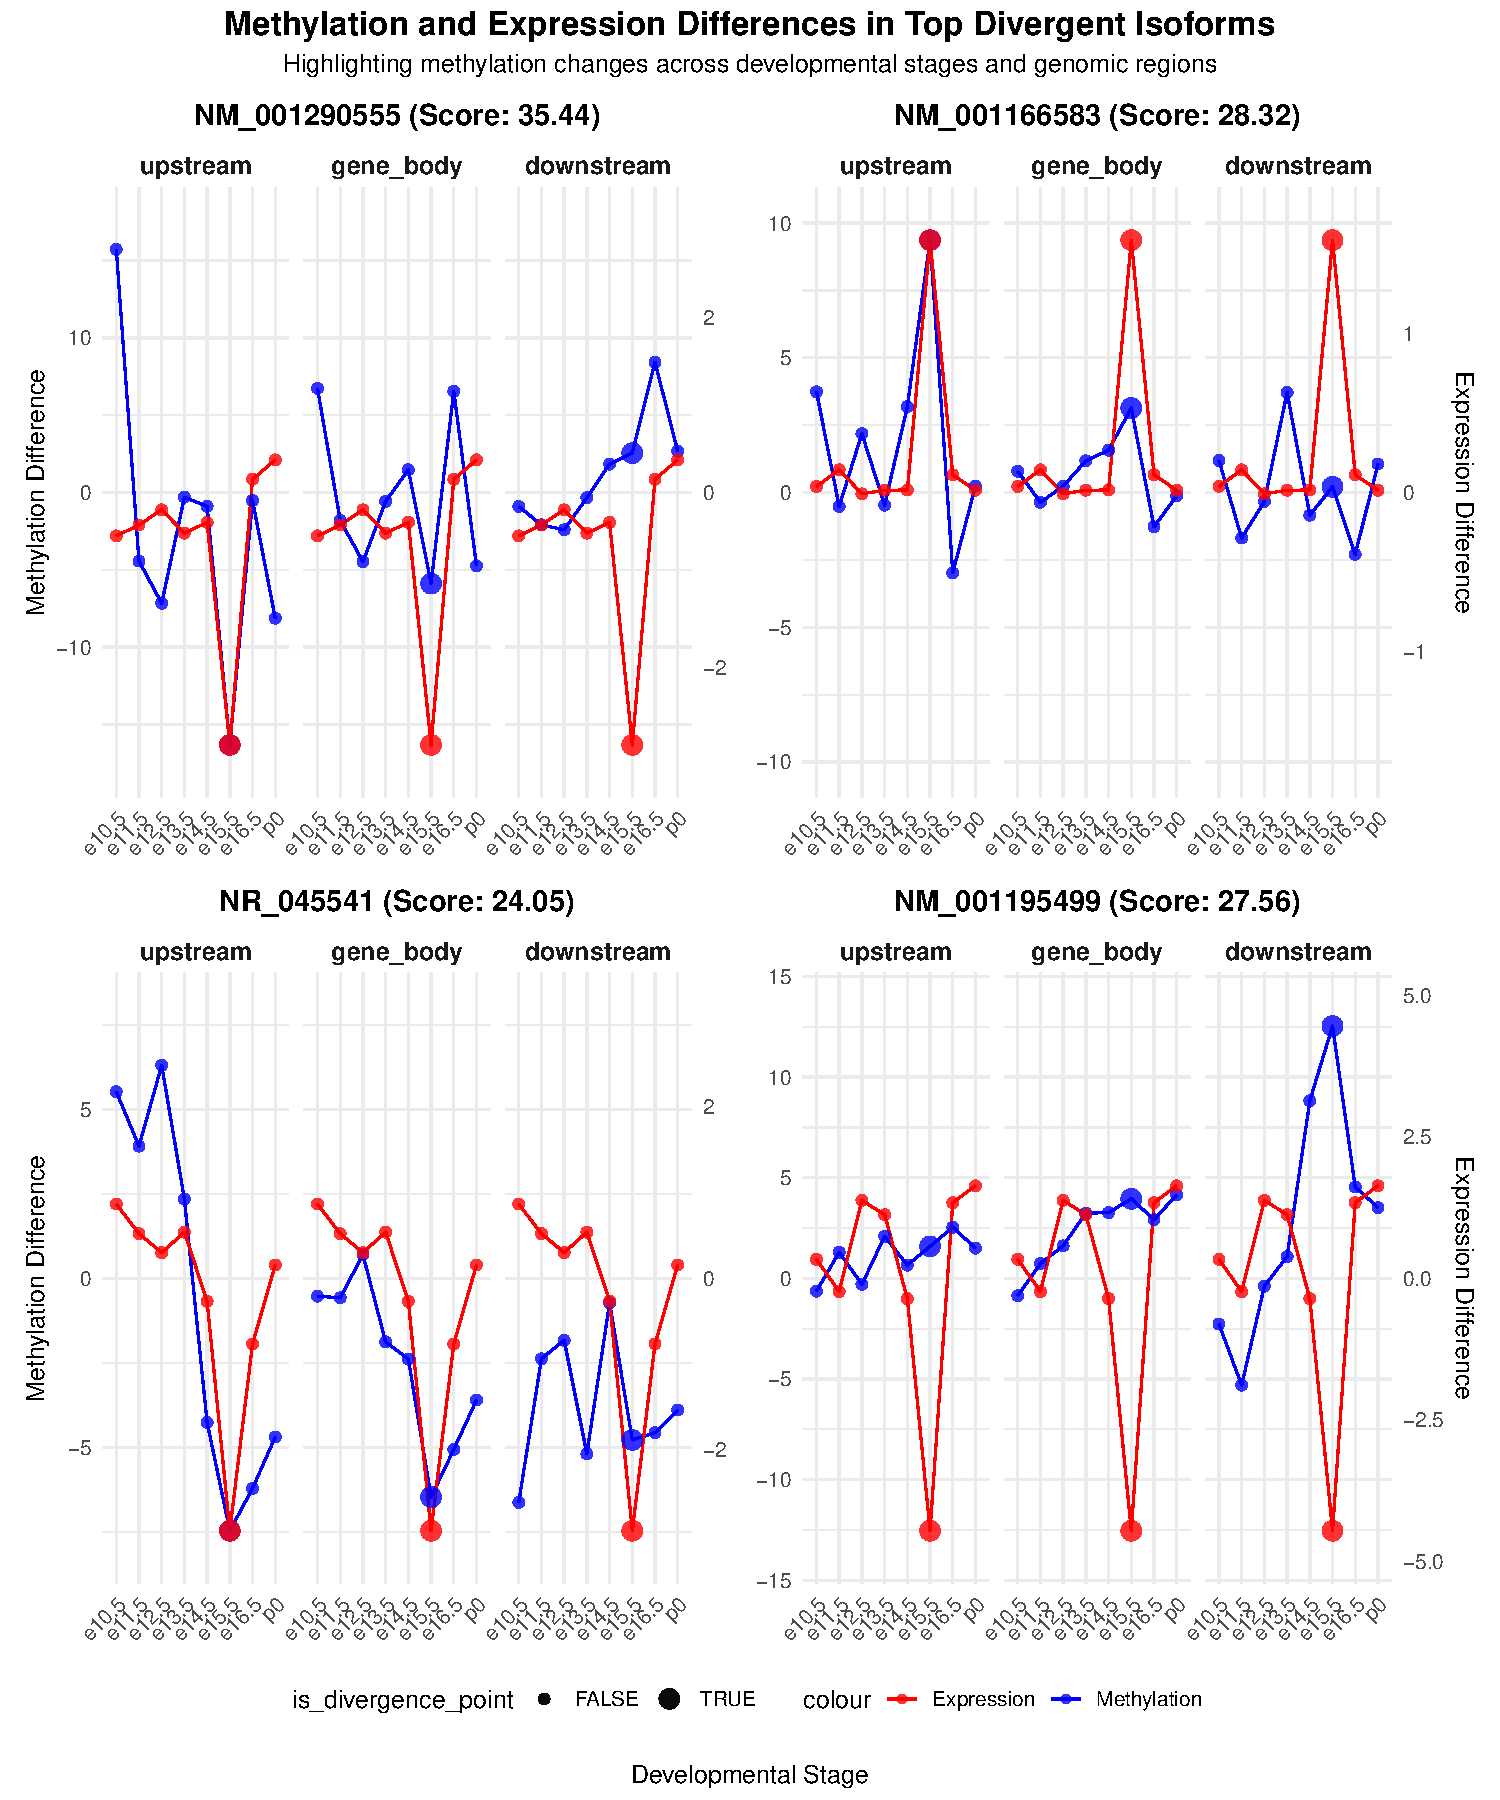
\includegraphics[width=0.92\textwidth]{figure_thesis_weighted_candidates.pdf}
\caption{\textbf{Methylation-weighted transcript candidates from the original ranking.} Rows show \textit{Pja1} NM\_001290555, \textit{Fam122b} NM\_001166583, \textit{Oprl1} NR\_045541 and \textit{Dclk2} NM\_001195499; columns show the 6-kb upstream window, gene body with 2-kb margins and 6-kb downstream window. Across E10.5--P0, blue and red trajectories are the midbrain-minus-forebrain methylation and transcript-expression differences, respectively, plotted on separate y-axis scales. Larger points identify stages classified as expression-divergence points by the original heuristic. ``Score'' is the inherited methylation-weighted divergence score used to rank 891 transcripts; it is not an analysis-wide test statistic or q-value.}
\label{fig:thesisweighted}
\end{figure}

\clearpage
\subsection*{Chromatin and methylation context}

These figures present exploratory chromatin-state and methylation summaries for the original transcript sets selected by the doctoral workflow before the analysis-wide reconstruction.

\begin{figure}[htbp]
\centering
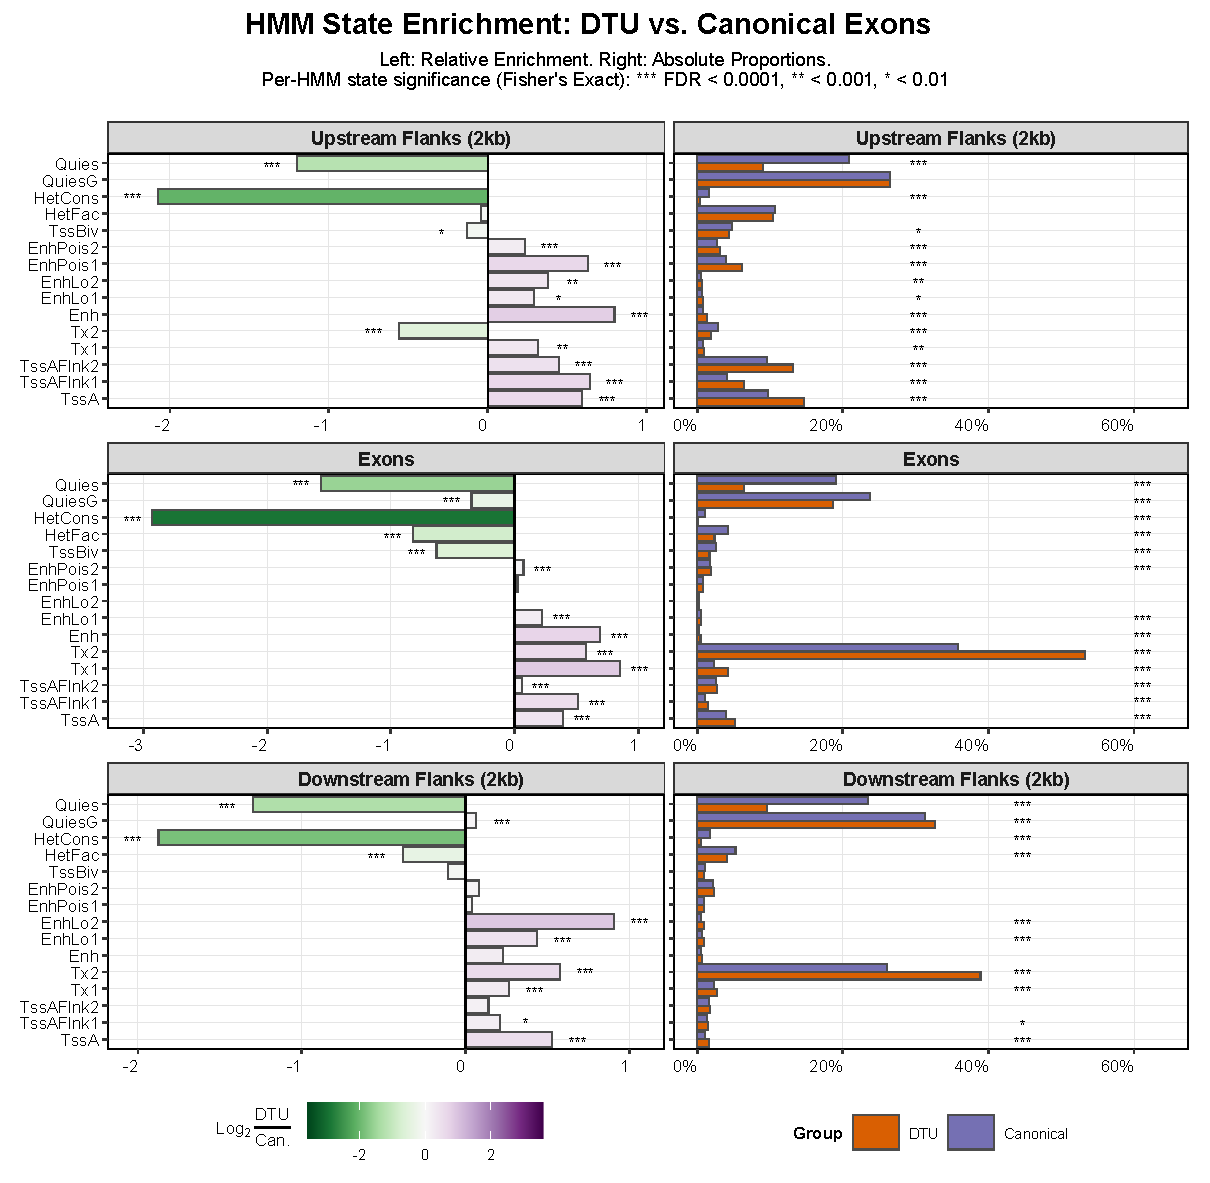
\includegraphics[width=0.94\textwidth]{figureS7_thesis_hmm_enrichment.pdf}
\caption{\textbf{Chromatin-state enrichment around DTU and comparison exons.} The analysis uses the 15-state E13.5 forebrain chromatin hidden Markov model. Rows are chromatin states and columns are the 2-kb upstream flank, exon and 2-kb downstream flank. Left panels show $\log_2$ enrichment of state overlap in the original DTU exon set relative to the non-DTU comparison set; right panels show the absolute percentage of features overlapping each state, with colour distinguishing the two sets. ``Canonical'' is the inherited label for the non-DTU comparison exons. Asterisks report per-state Fisher exact tests after FDR correction ($*$, FDR $<0.01$; $**$, FDR $<0.001$; $***$, FDR $<0.0001$).}
\label{fig:thesishmmenrichment}
\end{figure}

\begin{figure}[htbp]
\centering
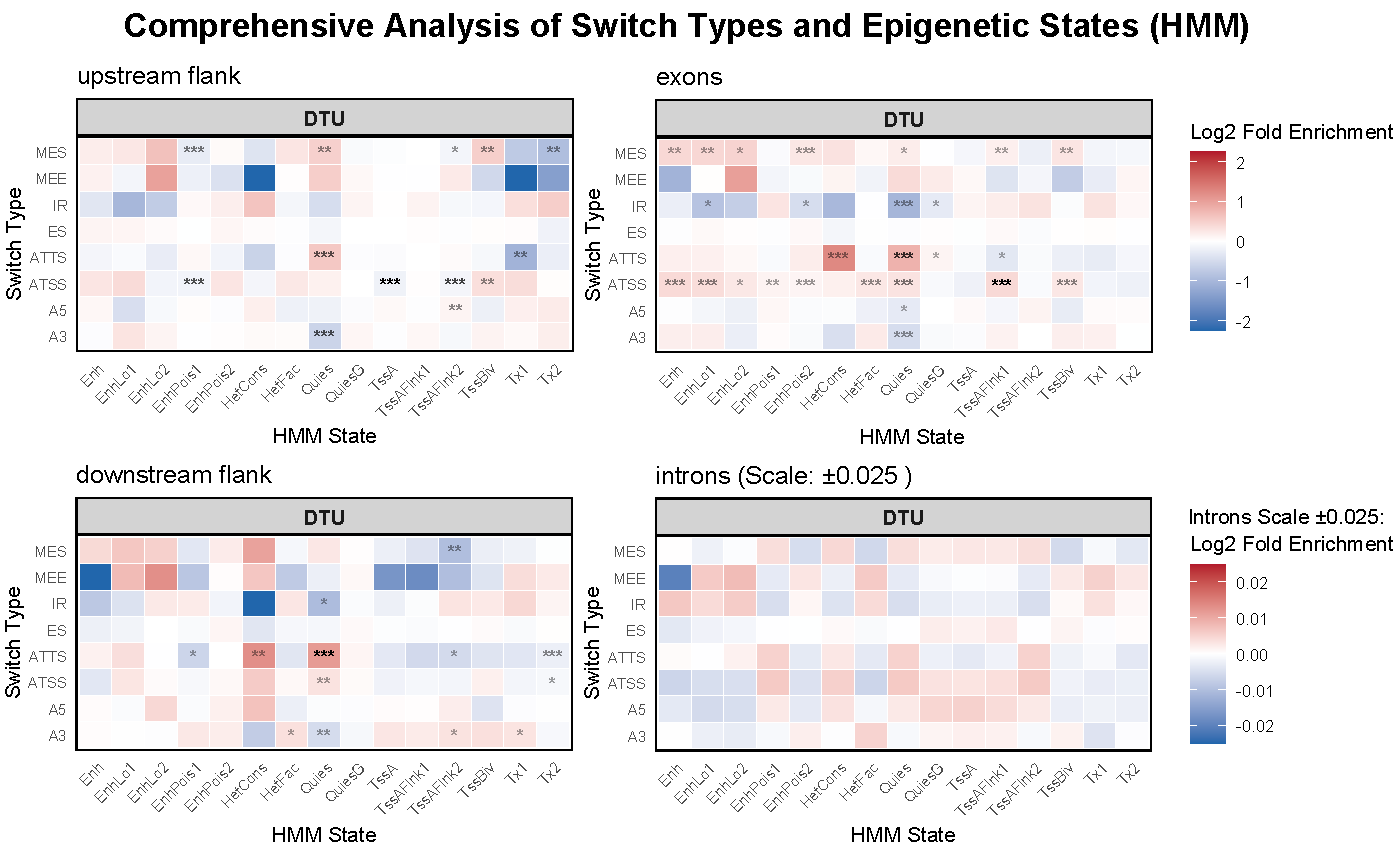
\includegraphics[width=0.94\textwidth]{figureS8_thesis_switch_hmm.pdf}
\caption{\textbf{Chromatin-state profiles by transcript-event annotation.} Four heatmaps show $\log_2$ enrichment of the 15 E13.5 forebrain hidden-Markov chromatin states in exons, introns, 2-kb upstream flanks and 2-kb downstream flanks. Rows are the pooled DTU set and the ES, MEE, MES, IR, A5, A3, ATSS and ATTS annotation groups defined in Figure~\ref{fig:thesissplicingidentity}; columns are the named chromatin states. Enrichment is relative to the original non-DTU comparison set, with positive values indicating over-representation. The intron panel uses the narrower scale printed in the figure ($\pm0.025$); the other panels use the common $\log_2$ scale. Asterisks reproduce the original FDR-coded state comparisons ($*$, FDR $<0.01$; $**$, FDR $<0.001$; $***$, FDR $<0.0001$).}
\label{fig:thesisswitchhmm}
\end{figure}

\begin{figure}[htbp]
\centering
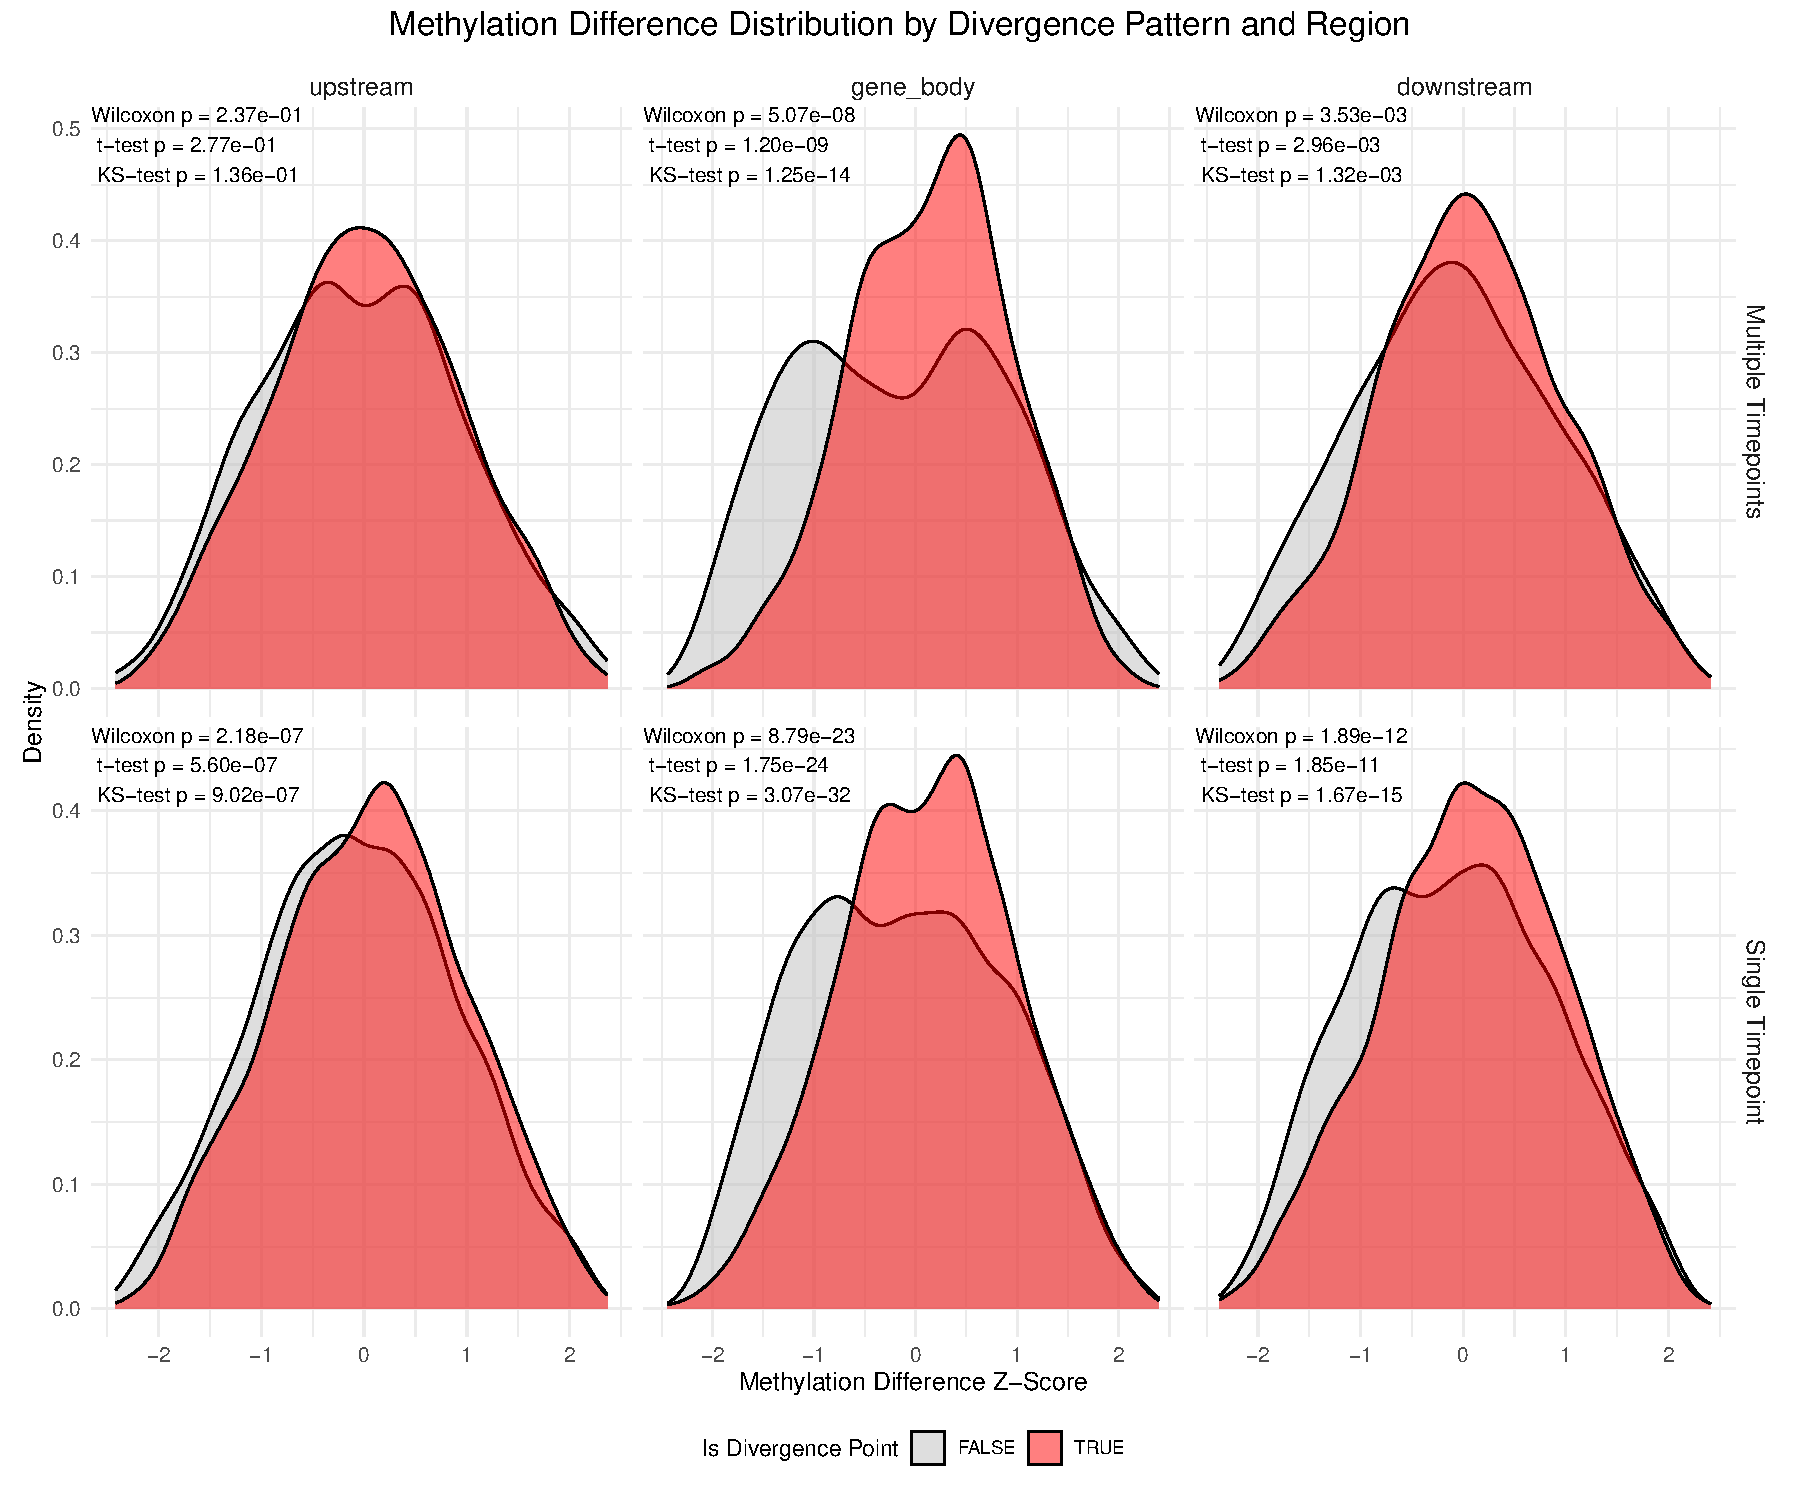
\includegraphics[width=0.94\textwidth]{figureS9_thesis_methylation_divergence.pdf}
\caption{\textbf{Methylation differences at divergent and non-divergent stages.} The observations derive from 891 transcripts selected by the original forebrain--midbrain expression-divergence heuristic. Columns are the 6-kb upstream window, gene body with 2-kb margins and 6-kb downstream window; rows separate transcripts divergent at multiple stages from those divergent at one stage. Within each facet, density curves compare transcript--stage methylation-difference Z-scores at stages labelled as expression-divergent (red) with the remaining stages (grey). The Z-score standardises the midbrain-minus-forebrain methylation difference within each transcript and genomic region across stages. Printed values are nominal two-sided Wilcoxon rank-sum, t-test and Kolmogorov--Smirnov $P$-values from the original workflow; no multiplicity correction across the six facets and three tests is encoded in the figure.}
\label{fig:thesismethdivergence}
\end{figure}

\fi
\end{document}
